\chapter{راهنمای استفاده از کلاس}
\thispagestyle{empty}
\section{مقدمه}
حروف‌چینی پروژه کارشناسی، پایان‌نامه یا رساله یکی از موارد پرکاربرد استفاده از زی‌پرشین است. از طرفی، یک پروژه، پایان‌نامه یا رساله،  احتیاج به تنظیمات زیادی از نظر صفحه‌آرایی  دارد که ممکن است برای
یک کاربر مبتدی، مشکل باشد. به همین خاطر، برای راحتی کار کاربر، کلاس حاضر با نام 
 \LRE{\verb!tabriz-thesis!}
 برای حروف‌چینی پروژه‌ها، پایان‌نامه‌ها و رساله‌های دانشگاه تبریز با استفاده از نرم‌افزار زی‌پرشین،  آماده شده است. این فایل به 
گونه‌ای طراحی شده است که کلیه خواسته‌های مورد نیاز  مدیریت تحصیلات تکمیلی دانشگاه تبریز را برآورده می‌کند و نیز، حروف‌چینی بسیاری
از قسمت‌های آن، به طور خودکار انجام می‌شود.

کلیه فایل‌های لازم برای حروف‌چینی با کلاس گفته شده، داخل پوشه‌ای به نام
 \LRE{\verb!tabriz-thesis!}
  قرار داده شده است. توجه داشته باشید که برای استفاده از این کلاس باید فونت‌های
\LRE{\verb!XB Niloofar!}،
 \verb!Yas!
 و
  \verb!IranNastaliq!
    روی سیستم شما نصب شده باشد.
\section{این همه فایل؟!}\label{sec2}
از آنجایی که یک پایان‌نامه یا رساله، یک نوشته بلند محسوب می‌شود، لذا اگر همه تنظیمات و مطالب پایان‌نامه را داخل یک فایل قرار بدهیم، باعث شلوغی
و سردرگمی می‌شود. به همین خاطر، قسمت‌های مختلف پایان‌نامه یا رساله  داخل فایل‌های جداگانه قرار گرفته است. مثلاً تنظیمات پایه‌ای کلاس، داخل فایل
\LRE{\verb!tabriz-thesis.cls!}، 
تنظیمات قابل تغییر توسط کاربر، داخل 
\verb!commands.tex!،
قسمت مشخصات فارسی پایان‌نامه، داخل 
\LRE{\verb!fa-title.tex!}،
مطالب فصل اول، داخل 
\verb!chapter1!
و ... قرار داده شده است. نکته مهمی که در اینجا وجود دارد این است که از بین این  فایل‌ها، فقط فایل 
\LRE{\verb!tabriz-thesis.tex!}
قابل اجرا است. یعنی بعد از تغییر فایل‌های دیگر، برای دیدن نتیجه تغییرات، باید این فایل را اجرا کرد. بقیه فایل‌ها به این فایل، کمک می‌کنند تا بتوانیم خروجی کار را ببینیم. اگر به فایل 
\LRE{\verb!tabriz-thesis.tex!}
دقت کنید، متوجه می‌شوید که قسمت‌های مختلف پایان‌نامه، توسط دستورهایی مانند 
\verb!input!
و
\verb!include!
به فایل اصلی، یعنی 
\LRE{\verb!tabriz-thesis.tex!}
معرفی شده‌اند. بنابراین، فایلی که همیشه با آن سروکار داریم، فایل 
\LRE{\verb!tabriz-thesis.tex!}
است.
در این فایل، فرض شده است که پایان‌نامه یا رساله، از ۳ فصل و یک پیوست، تشکیل شده است. با این حال، اگر
  پایان‌نامه یا رساله، بیشتر از ۳ فصل و یک پیوست است، باید خودتان فصل‌های بیشتر را به این فایل، اضافه کنید. این کار، بسیار ساده است. فرض کنید بخواهید یک فصل دیگر هم به پایان‌نامه، اضافه کنید. برای این کار، کافی است یک فایل با نام 
\verb!chapter4!
و با پسوند 
\verb!.tex!
بسازید و آن را داخل پوشه 
\LRE{\verb!tabriz-thesis!}
قرار دهید و سپس این فایل را با دستور 
\verb!\chapter{ نمونه‌ای از یک فصل}
\section{مدل‌های حرکت}\label{sec-model-motion}
بسته به کاربرد، حرکت مجموعه نقاط در فضای دلخواه از راه‌های مختلف نمایش داده می‌شود. حرکت می‌تواند به صورت صریح با توابع چندجمله‌ای، به صورت ضمنی با معادلات دیفرانسیلی، یا به صورت آماری با مدل‌های احتمالی نمایش داده شود. همان‌طورکه بعداً دیده خواهد شد، در مسائل وابسته به حرکت که نقاط مسئله به‌طور پیوسته در حال حرکت هستند، لازم است تا وضعیت نقاط در هر زمان با مجموعه‌ای از شرط‌های جبری مشخص شود. علاوه بر این نیاز است تا مسیر حرکت نقاط به‌گونه‌ای تعریف شود که تعداد دفعاتی که یک شرط جبری ممکن است نامعتبر ‌شود ثابت باشد. بدین منظور در این پایان‌نامه، فرض می‌شود که مسیر حرکت نقاط در صفحه به صورت  \textbf{حرکت‌های شبه‌جبری}\LTRfootnote{Pseudo algebraic motions} است. برای تعریف این نوع حرکت‌ها لازم است توابع شبه‌جبری تعریف شوند، که از تعریف زانگ\LTRfootnote{Zhang} مطرح شده در
 %\cite{z-kmps-00} 
 استفاده می‌شود. 

\begin{definition}\label{def-psdo-algb-func}
توابع پیوسته‌ی یک متغیره‌ی $f_{1}(x), f_{2}(x), ... , f_{m}(x)$، توابع شبه‌جبری از درجه‌ی حداکثر $s$ هستند، هرگاه برای هر تابع چندجمله‌ای $m$ متغیره‌ی $g$  از درجه‌ی $s_{1}$،  تابع  $$h(x) = g(f_{1}(x), f_{2}(x), ... , f_{m}(x))$$  متحد صفر باشد یا حداکثر $s \times s_{1}$  ریشه داشته باشد.
 \end{definition}
  برای نمونه، توابع چندجمله‌ای یا منطقی با درجه‌ی ثابت توابع شبه‌جبری هستند. یک مجموعه از نقاط دارای حرکت‌های شبه‌جبری از زمان هستند هرگاه مسیر حرکت آن‌ها با توابع شبه‌جبری از زمان توصیف شود. در ادامه، تعریف \ref{def-psdo-algb-func} با شرح یک مثال توضیح داده می‌شود. 
 
مسئله‌ی یک بعدی زیر که ترتیب $n$ نقطه‌ی در حال حرکت روی محور $x$ ها را گزارش می‌کند، درنظر بگیرید. هر نقطه‌ی $p_{i}$  دارای مسیر حرکت پیوسته‌ای از زمان است که با $f_{i}(t)$  نشان داده می‌شود و $t$ به زمان اشاره می‌کند. مقدار هر نقطه‌ی $p_{i}$  در زمان $t$، یعنی مولفه‌ی $x$ نقطه، با $v_{i}(t)$ نشان داده می‌شود. فرض کنید مجموعه توابع حرکت نقاط، یعنی $f_{1}(t), f_{2}(t), ... ، f_{n}(t)$،  توابع شبه‌جبری از درجه‌ی $s$ باشند و شرط‌های جبری برای تعیین موقعیت نقاط متحرک از نوع مقایسه تعریف شوند. اگر برای نشان دادن ترتیب هر دو نقطه‌ی متوالی $p_{i}$ و $p_{j}$ روی محور $x$ در زمان $t$، به‌طوری‌که $ v_{j}(t) > v_{i}(t)$ باشد، از شرط جبری $ v_{j}(t) - v_{i}(t) > 0$  استفاده شود، آنگاه با توجه به تعریف \mbox{\ref{def-psdo-algb-func}}، می‌توان تابع دو متغیره‌ی خطی $g(f_{j}, f_{i})(t) =  f_{j}(t) - f_{i}(t)$ (که طبق تعریف دارای $s_{1} = 1$ و $m = 2$ است)، را به عنوان تابع $h(t)$ درنظر گرفت و به این نتیجه رسید که تابع $h(t) = g(f_{j}, f_{i})(t)$ یا متحد صفر است یا دارای حداکثر $s \times 1$  ریشه است. این بدان معنی است که شرط جبری $ v_{j}(t) - v_{i}(t) > 0$ با گذشت زمان حداکثر به تعداد $s$ بار صفر می‌شود و متعاقباً تغییر علامت می‌دهد (تغییر ترتیب نقاط).
 
در تحلیل مسائلی که بعداً مطرح خواهند شد، بسیار اهمیت دارد که تعداد دفعاتی که شرط جبری مربوط به یک نقطه با گذشت زمان صفر می‌شود ثابت باشد. از آن‌جایی که در بیش‌تر مسائل شرط‌های جبری که برای تعیین وضعیت نقاط معرفی می‌شوند، چندجمله‌ای‌هایی از درجه‌ی کم، تعریف شده روی یک تعداد ثابت از نقاط هستند، فرض شبه‌جبری بودن حرکت نقاط کافی است تا برقراری این موضوع را تضمین کند. برای نمونه، در مثال بالا شرط‌های جبری (مقایسه‌ی دو مقدار) از درجه‌ی یک و تعریف شده روی دو نقطه هستند، بنابراین با فرض شبه‌جبری بودن حرکت نقاط، شرط جبری مربوط به یک نقطه همان تابع $g$ مطرح شده در تعریف \ref{def-psdo-algb-func} می‌شود که حداکثر به تعداد $s \times 1$  بار صفر خواهد شد ( $s$ یک عدد ثابت که درجه‌ی توابع شبه‌جبری حرکت را نشان می‌دهد). 

 \section{دنباله‌ی داونپورت-شینزل}\label{sec-DS-sequence}
 \begin{definition}
\label{def-DS-sequ}
یک $(n, s)$ دنباله‌ی داونپورت-شینزل\LTRfootnote{Davenport-Schinzel sequence}، که $n$ و $s$ اعداد صحیح مثبت هستند، یک دنباله‌ی ساخته شده از $n$ نماد با این خواص است که هیچ دو نماد مجاور در دنباله یکسان نیستند و این‌که برای هر دو نماد مجزای $a$ و $b$  حداکثر $s$  تناوب از آن‌ها در دنباله وجود دارد.
 \end{definition}
در تعریف بالا، منظور از تناوب $a$ و $b$ این است که نماد $b$ بعد از نماد $a$ و نماد $a$ بعد از نماد $b$ در دنباله ظاهر شود، ولی نه الزاماً مجاور به هم (کنار هم). مثلاً دنباله‌ی زیر، تشکیل شده از نمادهای $a, b, c, d$ را در نظر بگیرید: $$\underline{a}c\underline{b}dbc\underline{a}cd
\underline{b}\underline{a}dcdcadc\underline{b}$$ تعداد تناوب‌های $a$ و $b$ در دنباله، یعنی مجموع تعداد دفعاتی که $b$ بعد از $a$  و $a$ بعد از $b$ در دنباله ظاهر شده است، برابر با 5 است. با توجه به تعریف $(n, s)$ دنباله‌ی داونپورت-شینزل، می‌توان دریافت که با یک $n$ و $s$ معلوم (داده شده)، بسته به مقدارهای $n$ و $s$،  دنباله‌‌های داونپورت-شینزل متعددی می‌توان یافت، اما همگی دارای طول‌های متناهی هستند؛ زیرا با توجه به تعریف، امکان وجود دو نماد مجاور یکسان در دنباله نیست و نیز تعداد تناوب‌های هر دو نماد مجزا در دنباله به تعداد حداکثر $s$ محدود شده است. مثلاً برای $n = 3$ و $s = 2$ و نمادهای $a, b, c$،  طول  $(3, 2)$ دنباله‌های داونپورت-شینزل ممکن، حداکثر 5 است؛ زیرا هر دنباله با طول 6 یا بیش‌تر متشکل از این نمادها، یا حداقل برای یک جفت نماد مجزا دارای بیش از 2 تناوب خواهد بود یا دو نماد مجاور یکسان خواهد داشت و در نتیجه، شرایط تعریف یک $(3, 2)$ دنباله‌ی داونپورت-شینزل را نخواهد داشت، به عنوان مثال دنباله‌ی $abcbab$ که 3 تناوب از $a$ و $b$ را دارد. بنابراین طول طولانی‌ترین $(n, s)$ دنباله‌ی داونپورت-شینزل قابل تعریف خواهد بود 
و با $\lambda_{s}(n)$ نشان داده می‌شود. در ادامه به بیان اهمیت و کاربرد این دنباله‌ها در تحلیل مسائلی‌ مهم در هندسه‌ی محاسباتی پرداخته می‌شود.

اگر $\rbrace$ $f_{i}$ $ \lbrace$ $\cal F =$
  یک مجموعه از توابع باشد،  \textbf{ پوشش پایینی}\LTRfootnote{Lower envelope}  برای مجموعه $\cal F$  برابر تابع $\min f_{i}(x)$ است که با  $\Gamma(\cal F)$ نشان داده می‌شود.  به طور مشابه  $\max f_{i}(x)$ به عنوان \textbf{پوشش بالایی}\LTRfootnote{Upper envelope}  تعریف می‌شود. پیچیدگی $\Gamma(\cal F)$ نیز برابر با تعداد دفعاتی که تابع موجود در $\Gamma(\cal F)$ عوض می‌شود، یعنی تعداد نقاط شکست $\Gamma(\cal F)$ تعریف می‌شود. 

\begin{figure}[h]
\begin{center}
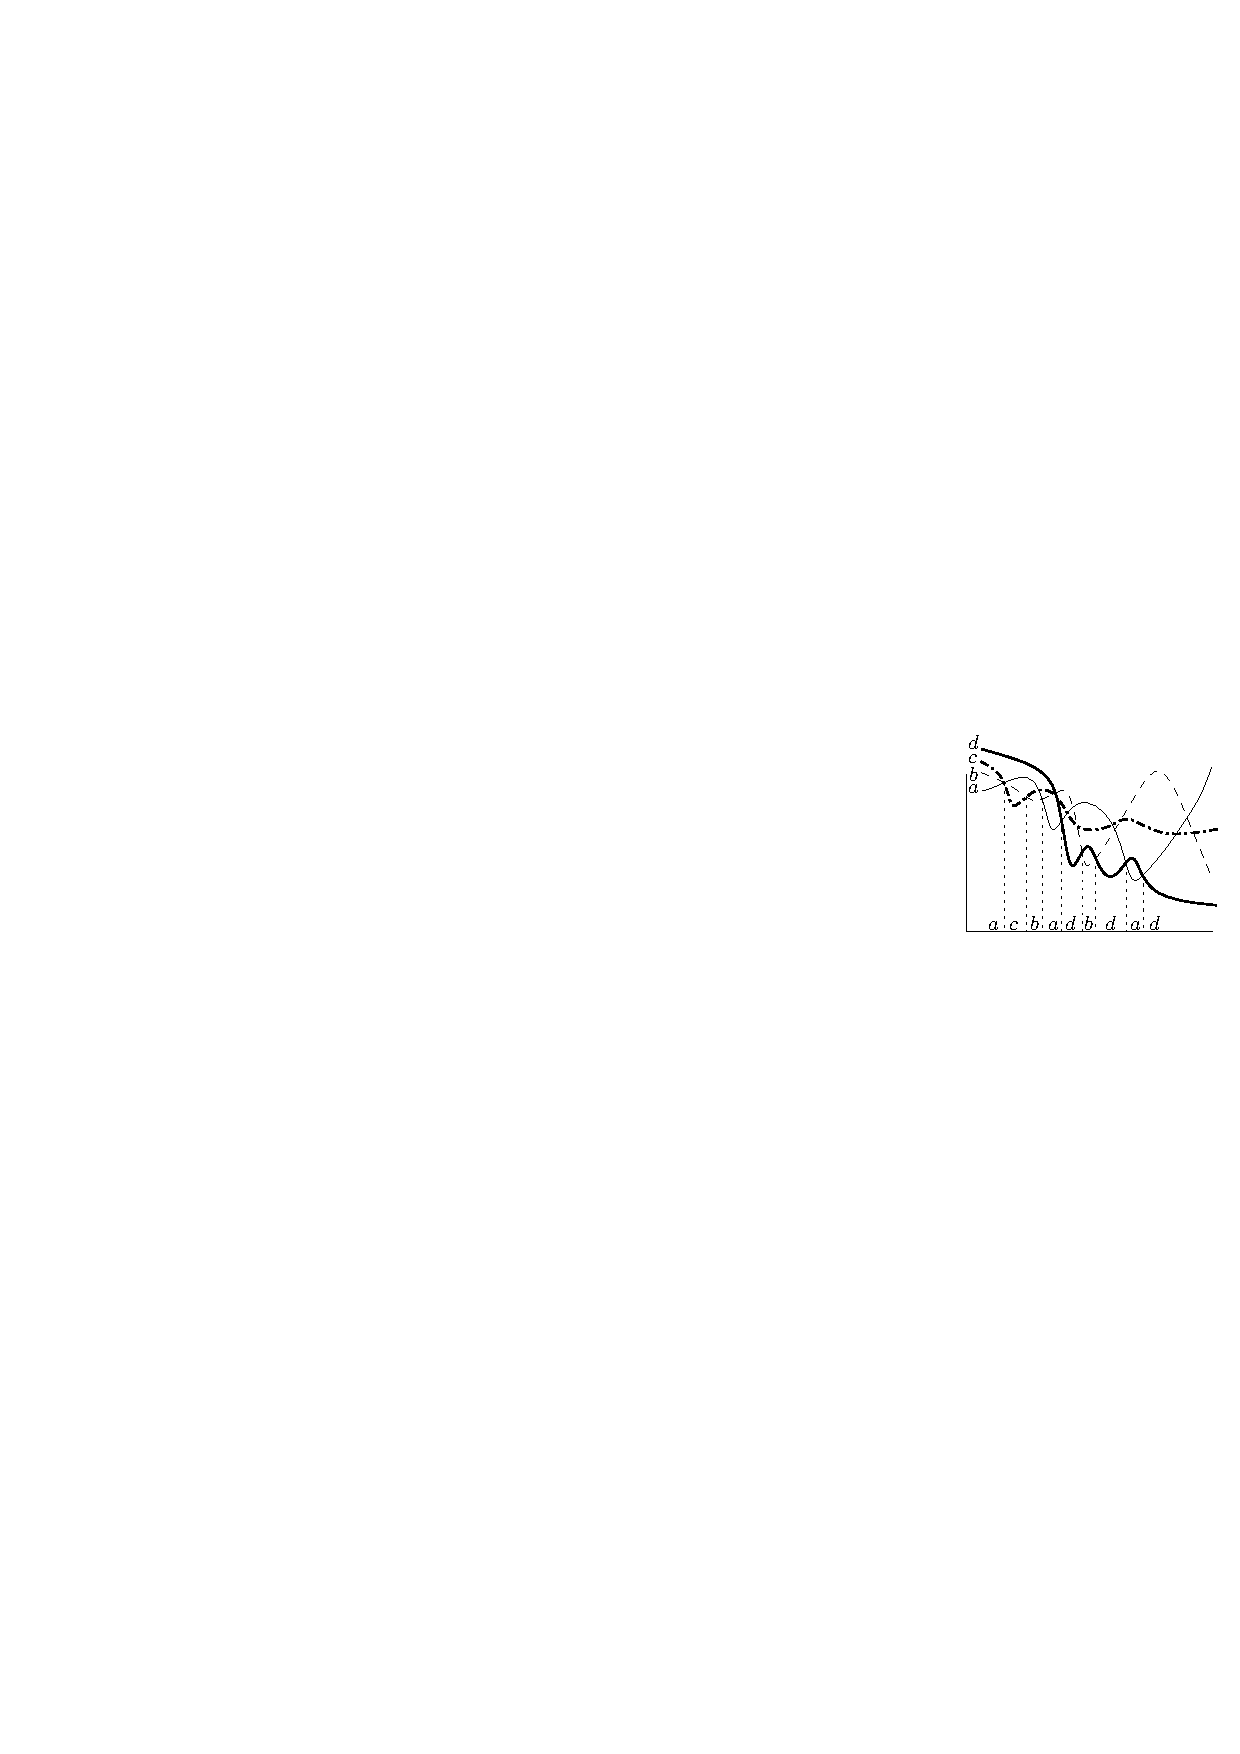
\includegraphics[width=0.5\textwidth]{DSsequence}
\end{center}
\caption{پوشش پایینی یک مجموعه از توابع متناظر با دنباله‌ای از نمادها}
\label{fig-DSsequence}
\end{figure}
اگر $\cal F$ مجموعه‌ای از $n$ تابع چندجمله‌ای با درجه‌ی $s$ باشد. با توجه به این‌که هر دو تابع چندجمله‌ای از درجه‌ی $s$ حداکثر در $s$ نقطه با یکدیگر برخورد می‌کنند (این بدان معنی است که حداکثر $s$ تناوب از هر دو تابع مجزا از $\cal F$  در $\Gamma(\cal F)$ وجود خواهد داشت) و نیز وجود دو تابع یکسان مجاور به هم در $\Gamma(\cal F)$ هم امکان ندارد، به‌راحتی می‌توان نتیجه گرفت که $\Gamma(\cal F)$ متناظر با یک $(n, s)$ دنباله‌ی داونپورت-شینزل است و پیچیدگی آن نیز، برابر با طول دنباله‌ی داونپورت-شینزل متناظر با آن خواهد شد. شکل \ref{fig-DSsequence} را ببینید. پس می‌توان گفت که پیچیدگی $\Gamma(\cal F)$ از مرتبه‌ی $O(\lambda_{s}(n))$ است. تمام نتایج به‌طور مشابه برای پیچیدگی پوشش بالایی نیز برقرار است. اگر دامنه‌ی تعریف $\Gamma(\cal F)$ در نظر گرفته شود و هر تابع چندجمله‌ای از $\cal F$  روی قسمتی از این دامنه (یک بازه مشخص از دامنه) تعریف شود، یعنی نمودار هر تابع تکه‌ای از نمودار آن تابع با دامنه نامحدود باشد، آنگاه پیچیدگی $ \Gamma(\cal F)$ برابر $O(\lambda_{s+2}(n))$ می‌شود \cite{sp-dssga-95}.
برای یک ثابت $s\geq 3$، $\lambda_{s}(n)$ یک تابع ابرخطی است اما خیلی آهسته رشد می‌کند. در ادامه قضیه‌ای بیان می‌شود که فرمول‌های مربوط به محاسبه  $\lambda_{s}(n)$ را بیان می‌کند. تابع $\alpha(n)$  به معکوس تابع آکرمان\LTRfootnote{Ackermann function} اشاره می‌کند \cite{sp-dssga-95}.


از آن جایی که $\alpha(n)$ تابعی است که بی‌نهایت آهسته رشد می‌کند (تقریبا برای مقادیر عملی و منطقاً بزرگ $n$ مقدار ثابت است)، بنابراین برای یک مقدار ثابت $s$، $\lambda_{s}(n)$ تقریبا خطی از $n$  است.   
%%%%%%%%%%%%%%%%%%%%%
 %%%%%%%%%%%%%%%%%%%
\section{پوشش‌های هندسی روی مجموعه نقاط}\label{sec-t-spann}
\subsection{شبکه‌های هندسی}
مجموعه‌ی $P$ شامل $n$ نقطه در فضای $\mathbb{R}^d$ را درنظر بگیرید، یک \textbf{شبکه‌ی متصل‌کننده‌ی نقاط} $P$\LTRfootnote{A network connecting the points of P}، یک گراف ${\cal G} = (P, E)$ با مجموعه رأس‌های $P$ و مجموعه یال‌های $E \subseteq P\times P$  است، به‌طوری‌که هر دو نقطه‌ی $p, q \in P$ با یک مسیر در $\cal G$ به‌هم متصل می‌شوند. یک \textbf{شبکه‌ی هندسی}\LTRfootnote{Geometric network} یا یک \textbf{گراف اقلیدسی}\LTRfootnote{Euclidean graph}، یک گراف وزن‌دار ${\cal G}$ است که رأس‌ها متناظر با نقاط در فضای اقلیدسی و وزن روی یال‌ها متناظر با فاصله‌‌ی اقلیدسی بین نقاط انتهایی آن یال است. شبکه‌های هندسی در واقع تعداد زیادی از شبکه‌های حقیقی موجود، مانند شبکه راه‌ها، شبکه مخابرات و غیره را مدل می‌کنند.
%\nocite{ns-gsn-07}

برای طراحی یک شبکه برای مجموعه‌ی مشخصی از نقاط، چندین معیار کیفی در نظر گرفته می‌شود. در زیر تعدادی از مهم‌ترین معیارهای کیفی برای ارزیابی شبکه‌های هندسی بیان شده است.
 \begin{enumerate}
\item
\textbf{اندازه}\LTRfootnote{Size}، به‌عنوان تعداد یال‌های شبکه تعریف می‌شود. در حالت کلی ترجیح داده می‌شود که شبکه‌ها تا جای ممکن اندازه‌ی کوچکی (خطی از تعداد نقاط) داشته باشند. 
\item
\textbf{وزن}\LTRfootnote{Weight}، به‌عنوان مجموع وزن یال‌های شبکه تعریف می‌شود. ازآن‌جایی‌که هر شبکه باید تمام نقاط را به‌هم وصل کند، درنتیجه وزن آن از پایین با وزن درخت پوشای کمینه کران‌دار می‌شود. وزن یک معیار خوب برای سنجش هزینه‌ی ساخت شبکه است. بنابراین، اغلب شبکه‌هایی با وزن کم مورد نظر هستند.
\item
\textbf{ضریب کشش}\LTRfootnote{Stretch factor}یا \textbf{تاخیر}\LTRfootnote{Dilation}  برای دو نقطه‌ی داده شده، برابر با نسبت کوتاه‌ترین مسیر (مسیر با وزن مینیمم) بین دو نقطه در شبکه، به فاصله‌ی آن دو نقطه بر اساس متر تعریف شده برای آن شبکه است (مثلاً این فاصله در متر اقلیدسی خط مستقیم متصل کننده‌ی دو نقطه است). ضریب کشش یک شبکه به‌عنوان بیش‌ترین ضریب کشش برای هر جفت از نقاط مجزا در شبکه تعریف می‌شود. در بسیاری از موارد، نیاز است که ضریب کشش شبکه با یک ثابت کوچک محدود شود (که حداقل باید یک باشد). شبکه‌ها با ضریب کشش حداکثر $t$، $t$-پوشش‌ها\LTRfootnote{t-Spanners} نامیده می‌شوند.
\item
\textbf{درجه}\LTRfootnote{Degree}،  بیش‌ترین تعداد یال‌های مجاور به هر نقطه در شبکه می‌باشد و اغلب نیاز است که با یک ثابت کوچک محدود شود. درجه‌ی محدود یک شبکه، به اندازه‌ی کوچک آن شبکه اشاره می‌کند، اما برعکس این مطلب لزوماً درست نیست.
\end{enumerate}
در حالت کلی، در زمان طراحی یک شبکه، آن‌چه که اهمیت زیادی دارد، اعمال ترکیبی از این معیارهای کیفی بر روی شبکه است و در زمان تحلیل شبکه نیز ویژگی‌های شبکه، نسبت به این معیارها سنجیده می‌شود. یکی از مسائل مهم در این زمینه، مطالعه‌ی شبکه‌هایی با ضریب کشش کم است (در ترکیب با دیگر ویژگی‌ها). ازجمله، در بسیاری از کاربردها مانند شبکه‌ی راه‌ها لازم است یک ارتباط سریع (مستقیم) بین هر جفت از نقاط در $P$ برقرار باشد (یعنی شبکه یک گراف کامل باشد) ولی این نیاز به خاطر هزینه‌های بالا، قابل اجرا شدن نیست. بنابراین نیاز به مطالعه‌ی شبکه‌هایی با ضریب کشش کم، منجر به شکل‌گیری مفهوم پوشش‌های هندسی می‌شود. این پوشش‌ها در واقع یک ساختار برای شبکه‌ها، زمانی که ارتباطات کوتاه بین نقاط اهمیت دارند را فراهم می‌کنند.
%%%%%%%%%%%%%%%%%%%%%%%%%%%%%%%%
\subsection{$t$-پوشش‌های هندسی}
 \begin{definition}
\label{def-t-spanner}
مجموعه‌ی $P$ شامل $n$ نقطه در فضای $\mathbb{R}^d$ و $t \geq 1$ را یک عدد حقیقی درنظر بگیرید. یک $t$-\textbf{پوشش}\LTRfootnote{t-spanner} برای $P$، یک گراف بدون ‌جهت $\cal G$ با مجموعه رأس‌های $P$  است، به‌طوری‌که کوتاه‌ترین مسیر بین هر دو نقطه‌ی $p$ و $q$ از $P$،  در $\cal G$ که با نماد $d_{\cal G}(p, q)$ نشان داده می‌شود، این شرط را داشته باشد:
$$d_{\cal G}(p, q) \leq t \cdot ||pq||.$$ هر مسیری که این شرط را برآورده سازد یک $t$-\textbf{مسیر}\LTRfootnote{t-path} بین $p$ و $q$ نامیده می‌شود.
\end{definition}
 برای هر عدد حقیقی $t^{'}$ که $t^{'} > t$ است، اگر $\cal G$ یک $t$-پوشش برای مجموعه نقاط $P$  باشد، بدیهی است که $\cal G$ یک $t^{'}$-پوشش نیز برای $P$ است. این، منجر به تعریف زیر می‌شود:
 \begin{definition}[\textbf{ضریب کشش}]
\label{def-strtch-factor}
مجموعه‌ی $P$ شامل $n$ نقطه در فضای $\mathbb{R}^d$ و $\cal G$ را یک گراف اقلیدسی با مجموعه رأس‌های $P$ درنظر بگیرید. ضریب کشش $\cal G$، کوچک‌ترین عدد حقیقی $t$ است به‌طوری‌که $\cal G$ یک $t$-پوشش از $P$ باشد.
\end{definition}
گراف کامل یک 1-پوشش است، اما تعداد مربعی یال دارد. درحقیقت، اگر فرض شود که هیچ سه نقطه‌ای از $P$  روی یک خط قرار ندارند، سپس گراف کامل تنها 1-پوشش برای $P$ است. بنابراین، در حالت کلی $t$-پوشش‌ها برای $t$ های بزرگ‌تر از یک بررسی می‌شوند. اما از آن‌جایی که در بسیاری از کاربردها، پوشش‌هایی با ارتباطات سریع (ضریب کشش کم) مورد نیاز هستند. بنابراین پوشش‌هایی با ضریب کشش نزدیک به یک، مورد مطالعه قرار می‌گیرند، یعنی $t = 1 + \varepsilon$،  برای مقادیر $\varepsilon$ مثبت و کوچک ($0 < \varepsilon < 1$). به این ترتیب، می‌توان با انتخاب مقادیر خیلی کوچک برای $\varepsilon$، مقدار $t$ را به یک نزدیک کرد، یعنی $t$-پوشش را به یک $1$-پوشش (گراف کامل) نزدیک کرد.
 %%%%%%%%%%%%%%%%%%%%%%%%%

 \section{ یک پوشش هندسی وابسته به حرکت در صفحه}
در این فصل یک $1 + \varepsilon$-پوشش ساده با اندازه‌ی خطی، برای یک مجموعه از $n$ نقطه در صفحه معرفی می‌شود. این پوشش زمانی‌که نقاط آن حرکت می‌کنند، می‌تواند به‌صورتی کارا نگهداری شود. فرض می‌شود که مسیر حرکت نقاط با توابع شبه‌جبری از درجه‌ی حداکثر $s$ توصیف می‌شوند (بخش \ref{sec-model-motion} را ببینید). لازم به ذکر است که مطالب این فصل بر اساس مقاله‌ی آبام\LTRfootnote{Abam} و همکارانش \cite{abg-seks-10} تنظیم شده است. \section{کارهای مرتبط}
یک $1 + \varepsilon$-پوشش را درنظر بگیرید. برای جزئیات بیش‌تر در مورد پوشش‌ها می‌توانید بخش \ref{sec-t-spann} را ببینید. هنگامی که نقاط پوشش دارای حرکت پیوسته‌ای از زمان باشند، پوشش به‌طور پیوسته از زمان تغییر می‌کند، اما تنها در لحظه‌های مشخصی نیاز به به‌روزرسانی خواهد داشت، تا همچنان در تمام زمان‌ها یک $1 + \varepsilon$-پوشش باقی بماند. در فصل 2 بیان شد که این لحظات رویداد نامیده می‌شوند. از آن‌جایی که کارایی و پاسخ‌گویی، از مهم‌ترین معیارها برای ارزیابی کیفیت ساختارهای وابسته به حرکت هستند، هدف، طراحی پوششی است که تعداد رویدادها و نیز زمان پاسخ‌گویی آن، کم باشد. همان‌طورکه در فصل 2 بیان شد، در حالت ایده‌ال، تعداد رویدادها باید نزدیک به کم‌ترین تعداد رویدادهایی که برای نگهداری ساختار لازم است باشد. برای پوشش‌ها، این بدین معنی است که تعداد رویدادها باید $O(n^{2})$ باشد؛ زیرا مجموعه‌های $n$ تایی از نقاط که به‌صورت خطی در صفحه حرکت می‌کنند وجود دارند، که برای هر $1 + \varepsilon$-پوشش باید $\Omega(n^{2}/(1 + \varepsilon)^{2})$ رویداد پردازش شود.
% \cite{ggn-dsa-06}. 
زمان پاسخ‌گویی نیز در حالت ایده‌ال باید چندلگاریتمی باشد.

\subsection{تحلیل ضریب کشش و اندازه‌ی پوشش}  \label{subsec-span-ratio}
در این زیربخش ثابت خواهد ‌شد که اگر زاویه‌های $\phi$ و $\varphi$ به‌گونه‌ای انتخاب شوند که شرط‌های 
%\begin{latin}
\begin{equation}\label{eq-rd-first}
(\cos \phi - \sin \phi) \geq 1/(1 + \varepsilon) 
\end{equation} 
%\end{latin}
و
 \begin{equation}\label{eq-rd-sec}(\sin(\phi/2)/\sin(\varphi/2)) \geq 1 + 2/\varepsilon \end{equation}
 برقرار باشند، آنگاه ${\cal DDS}(P)$ یک $1 + \varepsilon$-پوشش برای مجموعه نقاط $P$ خواهد بود. این شرط‌ها می‌توانند با تنظیم زوایای $\phi$ و $\varphi$ به‌صورت  $ \phi = \arcsin \frac{\varepsilon}{2(1+\varepsilon)}$ و $ \varphi = 2\arcsin \frac{\varepsilon^{2}}{4(1+\varepsilon)(2+\varepsilon)}$  به‌دست آیند. همواره فرض می‌شود که $\varphi <\phi$.  
\begin{observation}
\label{obsr-phi}
اگر $ \phi = \arcsin \frac{\varepsilon}{2(1+\varepsilon)}$ برقرار باشد آنگاه $0 < \phi < \dfrac{\pi}{6}$.
\end{observation}
\begin{proof}
از آن‌جایی‌که، $\dfrac{\varepsilon}{2(1+\varepsilon)} < \dfrac{1}{2}$  و تابع $\arcsin$ در بازه $ (0, \pi/2)$ یک تابع صعودی است، بنابراین،
 $$0 < \phi = \arcsin \frac{\varepsilon}{2(1+\varepsilon)} < \arcsin \frac{1}{2} = \dfrac{\pi}{6}.$$
\end{proof}
\begin{observation}
\label{obsr-angles}
با انتخاب $ \phi = \arcsin \frac{\varepsilon}{2(1+\varepsilon)}$ و $\varphi = 2\arcsin \frac{\varepsilon^{2}}{4(1+\varepsilon)(2+\varepsilon)}$ دو شرط \ref{eq-rd-first} و \ref{eq-rd-sec} برقرار است.
\end{observation}
مشتق\index{مشتق} تابع $f$، تابعی است که با علامت $f'$ نشان داده می‌شود و مقدار آن در هر عدد $x$ واقع در دامنهٔ $f$
به صورت 
\begin{align}\label{bderi1}
f'(x)=\lim_{\Delta x\rightarrow 0}\dfrac{f(x+\Delta x) - f(x)}{\Delta x}
\end{align}
\ysymbol{$f'(x)$}{مشتق تابع $f$ در نقطهٔ $x$}
تعریف می‌شود؛ به شرطی که حد فوق وجود داشته باشد.

اگر $f$ روی بازهٔ $[a,b]$ هموار باشد، طول منحنی $y=f(x)$ از $a$ تا $b$ برابر است با
\begin{align}\label{10eq6}
L=\int_a^b \sqrt{1+\Big(\dfrac{dy}{dx}\Big)^2}dx=\int_a^b \sqrt{1+(f'(x))^2}dx.
\ysymbol{$L$}{طول منحنی}
\end{align}

اگر تابع $f$ در $x_1$ تعریف شده باشد، آنگاه مشتق راست $f$ در $x_1$ با $f'_{+}(x_1)$ 
\ysymbol{$f'_{+}(x)$}{مشتق راست  $f$ در نقطهٔ $x$}
نشان داده می‌شود و به صورت 
\begin{align}
f'_{+}(x_1)=\lim_{\Delta x\rightarrow 0^{+}}\dfrac{f(x_1+\Delta x) - f(x_1)}{\Delta x}
\end{align}
و یا به عبارت دیگر،
تعریف می‌شود؛ به شرطی که این حدود موجود باشند.

\begin{example}
نمونه مثال
\end{example}
\begin{proposition}
نمونه گزاره
\end{proposition}
\begin{corollary}
نمونه نتیجه
\end{corollary}

\begin{remark}
نمونه ملاحظه
\end{remark}


!
داخل فایل
\LRE{\verb!tabriz-thesis.tex!}
و بعد از دستور
\verb!\chapter{راهنمای استفاده از کلاس \lr{yazd-thesis}}
\section{مقدمه}
حروف‌چینی پایان‌نامه یا رساله یکی از موارد پرکاربرد استفاده از زی‌پرشین است. از طرفی، یک  پایان‌نامه یا رساله،  احتیاج به تنظیمات زیادی از نظر صفحه‌آرایی  دارد که ممکن است برای
یک کاربر مبتدی، مشکل باشد. به همین خاطر، برای راحتی کار کاربر، کلاس حاضر با نام 
 \LRE{\verb!yazd-thesis!}
 برای حروف‌چینی پروژه‌ها، پایان‌نامه‌ها و رساله‌های دانشگاه یزد با استفاده از نرم‌افزار زی‌پرشین،  آماده شده است. این فایل به 
گونه‌ای طراحی شده است که کلیه خواسته‌های مورد نیاز  مدیریت تحصیلات تکمیلی دانشگاه یزد را برآورده می‌کند. همچنین حروف‌چینی بسیاری
از قسمت‌های آن، به طور خودکار انجام می‌شود.

کلیه فایل‌های لازم برای حروف‌چینی با کلاس گفته شده، داخل پوشه‌ای به نام
 \LRE{\verb!yazd-thesis!}
  قرار داده شده است. توجه داشته باشید که برای استفاده از این کلاس باید فونت
 \verb!Yas!
    روی سیستم شما نصب شده باشد.
\section{این همه فایل؟!}\label{sec2}
از آنجایی که یک پایان‌نامه یا رساله، یک نوشته بلند محسوب می‌شود، لذا اگر همه تنظیمات و مطالب پایان‌نامه را داخل یک فایل قرار بدهیم، باعث شلوغی
و سردرگمی می‌شود. به همین خاطر، قسمت‌های مختلف پایان‌نامه یا رساله  داخل فایل‌های جداگانه قرار گرفته است. مثلاً تنظیمات  کلاس داخل فایل
\LRE{\verb!yazd-thesis.cls!}، 
قسمت مشخصات فارسی پایان‌نامه داخل 
\LRE{\verb!fainfo.tex!}،
مطالب فصل اول، داخل 
\verb!chapter1!
و ... قرار داده شده است. نکته مهمی که در اینجا وجود دارد این است که از بین این  فایل‌ها، فقط فایل 
\LRE{\verb!yazd-thesis.tex!}
قابل اجرا است. یعنی بعد از تغییر فایل‌های دیگر، برای دیدن نتیجه تغییرات، باید این فایل را اجرا کرد. بقیه فایل‌ها به این فایل، کمک می‌کنند تا بتوانیم خروجی کار را ببینیم. اگر به فایل 
\LRE{\verb!yazd-thesis.tex!}
دقت کنید، متوجه می‌شوید که قسمت‌های مختلف پایان‌نامه، توسط دستورهایی مانند 
\verb!input!
و
\verb!include!
به فایل اصلی، یعنی 
\LRE{\verb!yazd-thesis.tex!}
معرفی شده‌اند. بنابراین، فایلی که همیشه با آن سروکار داریم، فایل 
\LRE{\verb!yazd-thesis.tex!}
است.
در این فایل، فرض شده است که پایان‌نامه یا رساله، از ۳ فصل و یک پیوست، تشکیل شده است. با این حال، اگر
  پایان‌نامه یا رساله، بیشتر از ۳ فصل و یک پیوست است، باید خودتان فصل‌های بیشتر را به این فایل، اضافه کنید. این کار، بسیار ساده است. فرض کنید بخواهید یک فصل دیگر هم به پایان‌نامه، اضافه کنید. برای این کار، کافی است یک فایل با نام 
\verb!chapter4!
و با پسوند 
\verb!.tex!
بسازید و آن را داخل پوشه 
\LRE{\verb!yazd-thesis!}
قرار دهید و سپس این فایل را با دستور 
\verb!\chapter{ نمونه‌ای از یک فصل}
\section{مدل‌های حرکت}\label{sec-model-motion}
بسته به کاربرد، حرکت مجموعه نقاط در فضای دلخواه از راه‌های مختلف نمایش داده می‌شود. حرکت می‌تواند به صورت صریح با توابع چندجمله‌ای، به صورت ضمنی با معادلات دیفرانسیلی، یا به صورت آماری با مدل‌های احتمالی نمایش داده شود. همان‌طورکه بعداً دیده خواهد شد، در مسائل وابسته به حرکت که نقاط مسئله به‌طور پیوسته در حال حرکت هستند، لازم است تا وضعیت نقاط در هر زمان با مجموعه‌ای از شرط‌های جبری مشخص شود. علاوه بر این نیاز است تا مسیر حرکت نقاط به‌گونه‌ای تعریف شود که تعداد دفعاتی که یک شرط جبری ممکن است نامعتبر ‌شود ثابت باشد. بدین منظور در این پایان‌نامه، فرض می‌شود که مسیر حرکت نقاط در صفحه به صورت  \textbf{حرکت‌های شبه‌جبری}\LTRfootnote{Pseudo algebraic motions} است. برای تعریف این نوع حرکت‌ها لازم است توابع شبه‌جبری تعریف شوند، که از تعریف زانگ\LTRfootnote{Zhang} مطرح شده در
 %\cite{z-kmps-00} 
 استفاده می‌شود. 

\begin{definition}\label{def-psdo-algb-func}
توابع پیوسته‌ی یک متغیره‌ی $f_{1}(x), f_{2}(x), ... , f_{m}(x)$، توابع شبه‌جبری از درجه‌ی حداکثر $s$ هستند، هرگاه برای هر تابع چندجمله‌ای $m$ متغیره‌ی $g$  از درجه‌ی $s_{1}$،  تابع  $$h(x) = g(f_{1}(x), f_{2}(x), ... , f_{m}(x))$$  متحد صفر باشد یا حداکثر $s \times s_{1}$  ریشه داشته باشد.
 \end{definition}
  برای نمونه، توابع چندجمله‌ای یا منطقی با درجه‌ی ثابت توابع شبه‌جبری هستند. یک مجموعه از نقاط دارای حرکت‌های شبه‌جبری از زمان هستند هرگاه مسیر حرکت آن‌ها با توابع شبه‌جبری از زمان توصیف شود. در ادامه، تعریف \ref{def-psdo-algb-func} با شرح یک مثال توضیح داده می‌شود. 
 
مسئله‌ی یک بعدی زیر که ترتیب $n$ نقطه‌ی در حال حرکت روی محور $x$ ها را گزارش می‌کند، درنظر بگیرید. هر نقطه‌ی $p_{i}$  دارای مسیر حرکت پیوسته‌ای از زمان است که با $f_{i}(t)$  نشان داده می‌شود و $t$ به زمان اشاره می‌کند. مقدار هر نقطه‌ی $p_{i}$  در زمان $t$، یعنی مولفه‌ی $x$ نقطه، با $v_{i}(t)$ نشان داده می‌شود. فرض کنید مجموعه توابع حرکت نقاط، یعنی $f_{1}(t), f_{2}(t), ... ، f_{n}(t)$،  توابع شبه‌جبری از درجه‌ی $s$ باشند و شرط‌های جبری برای تعیین موقعیت نقاط متحرک از نوع مقایسه تعریف شوند. اگر برای نشان دادن ترتیب هر دو نقطه‌ی متوالی $p_{i}$ و $p_{j}$ روی محور $x$ در زمان $t$، به‌طوری‌که $ v_{j}(t) > v_{i}(t)$ باشد، از شرط جبری $ v_{j}(t) - v_{i}(t) > 0$  استفاده شود، آنگاه با توجه به تعریف \mbox{\ref{def-psdo-algb-func}}، می‌توان تابع دو متغیره‌ی خطی $g(f_{j}, f_{i})(t) =  f_{j}(t) - f_{i}(t)$ (که طبق تعریف دارای $s_{1} = 1$ و $m = 2$ است)، را به عنوان تابع $h(t)$ درنظر گرفت و به این نتیجه رسید که تابع $h(t) = g(f_{j}, f_{i})(t)$ یا متحد صفر است یا دارای حداکثر $s \times 1$  ریشه است. این بدان معنی است که شرط جبری $ v_{j}(t) - v_{i}(t) > 0$ با گذشت زمان حداکثر به تعداد $s$ بار صفر می‌شود و متعاقباً تغییر علامت می‌دهد (تغییر ترتیب نقاط).
 
در تحلیل مسائلی که بعداً مطرح خواهند شد، بسیار اهمیت دارد که تعداد دفعاتی که شرط جبری مربوط به یک نقطه با گذشت زمان صفر می‌شود ثابت باشد. از آن‌جایی که در بیش‌تر مسائل شرط‌های جبری که برای تعیین وضعیت نقاط معرفی می‌شوند، چندجمله‌ای‌هایی از درجه‌ی کم، تعریف شده روی یک تعداد ثابت از نقاط هستند، فرض شبه‌جبری بودن حرکت نقاط کافی است تا برقراری این موضوع را تضمین کند. برای نمونه، در مثال بالا شرط‌های جبری (مقایسه‌ی دو مقدار) از درجه‌ی یک و تعریف شده روی دو نقطه هستند، بنابراین با فرض شبه‌جبری بودن حرکت نقاط، شرط جبری مربوط به یک نقطه همان تابع $g$ مطرح شده در تعریف \ref{def-psdo-algb-func} می‌شود که حداکثر به تعداد $s \times 1$  بار صفر خواهد شد ( $s$ یک عدد ثابت که درجه‌ی توابع شبه‌جبری حرکت را نشان می‌دهد). 

 \section{دنباله‌ی داونپورت-شینزل}\label{sec-DS-sequence}
 \begin{definition}
\label{def-DS-sequ}
یک $(n, s)$ دنباله‌ی داونپورت-شینزل\LTRfootnote{Davenport-Schinzel sequence}، که $n$ و $s$ اعداد صحیح مثبت هستند، یک دنباله‌ی ساخته شده از $n$ نماد با این خواص است که هیچ دو نماد مجاور در دنباله یکسان نیستند و این‌که برای هر دو نماد مجزای $a$ و $b$  حداکثر $s$  تناوب از آن‌ها در دنباله وجود دارد.
 \end{definition}
در تعریف بالا، منظور از تناوب $a$ و $b$ این است که نماد $b$ بعد از نماد $a$ و نماد $a$ بعد از نماد $b$ در دنباله ظاهر شود، ولی نه الزاماً مجاور به هم (کنار هم). مثلاً دنباله‌ی زیر، تشکیل شده از نمادهای $a, b, c, d$ را در نظر بگیرید: $$\underline{a}c\underline{b}dbc\underline{a}cd
\underline{b}\underline{a}dcdcadc\underline{b}$$ تعداد تناوب‌های $a$ و $b$ در دنباله، یعنی مجموع تعداد دفعاتی که $b$ بعد از $a$  و $a$ بعد از $b$ در دنباله ظاهر شده است، برابر با 5 است. با توجه به تعریف $(n, s)$ دنباله‌ی داونپورت-شینزل، می‌توان دریافت که با یک $n$ و $s$ معلوم (داده شده)، بسته به مقدارهای $n$ و $s$،  دنباله‌‌های داونپورت-شینزل متعددی می‌توان یافت، اما همگی دارای طول‌های متناهی هستند؛ زیرا با توجه به تعریف، امکان وجود دو نماد مجاور یکسان در دنباله نیست و نیز تعداد تناوب‌های هر دو نماد مجزا در دنباله به تعداد حداکثر $s$ محدود شده است. مثلاً برای $n = 3$ و $s = 2$ و نمادهای $a, b, c$،  طول  $(3, 2)$ دنباله‌های داونپورت-شینزل ممکن، حداکثر 5 است؛ زیرا هر دنباله با طول 6 یا بیش‌تر متشکل از این نمادها، یا حداقل برای یک جفت نماد مجزا دارای بیش از 2 تناوب خواهد بود یا دو نماد مجاور یکسان خواهد داشت و در نتیجه، شرایط تعریف یک $(3, 2)$ دنباله‌ی داونپورت-شینزل را نخواهد داشت، به عنوان مثال دنباله‌ی $abcbab$ که 3 تناوب از $a$ و $b$ را دارد. بنابراین طول طولانی‌ترین $(n, s)$ دنباله‌ی داونپورت-شینزل قابل تعریف خواهد بود 
و با $\lambda_{s}(n)$ نشان داده می‌شود. در ادامه به بیان اهمیت و کاربرد این دنباله‌ها در تحلیل مسائلی‌ مهم در هندسه‌ی محاسباتی پرداخته می‌شود.

اگر $\rbrace$ $f_{i}$ $ \lbrace$ $\cal F =$
  یک مجموعه از توابع باشد،  \textbf{ پوشش پایینی}\LTRfootnote{Lower envelope}  برای مجموعه $\cal F$  برابر تابع $\min f_{i}(x)$ است که با  $\Gamma(\cal F)$ نشان داده می‌شود.  به طور مشابه  $\max f_{i}(x)$ به عنوان \textbf{پوشش بالایی}\LTRfootnote{Upper envelope}  تعریف می‌شود. پیچیدگی $\Gamma(\cal F)$ نیز برابر با تعداد دفعاتی که تابع موجود در $\Gamma(\cal F)$ عوض می‌شود، یعنی تعداد نقاط شکست $\Gamma(\cal F)$ تعریف می‌شود. 

\begin{figure}[h]
\begin{center}
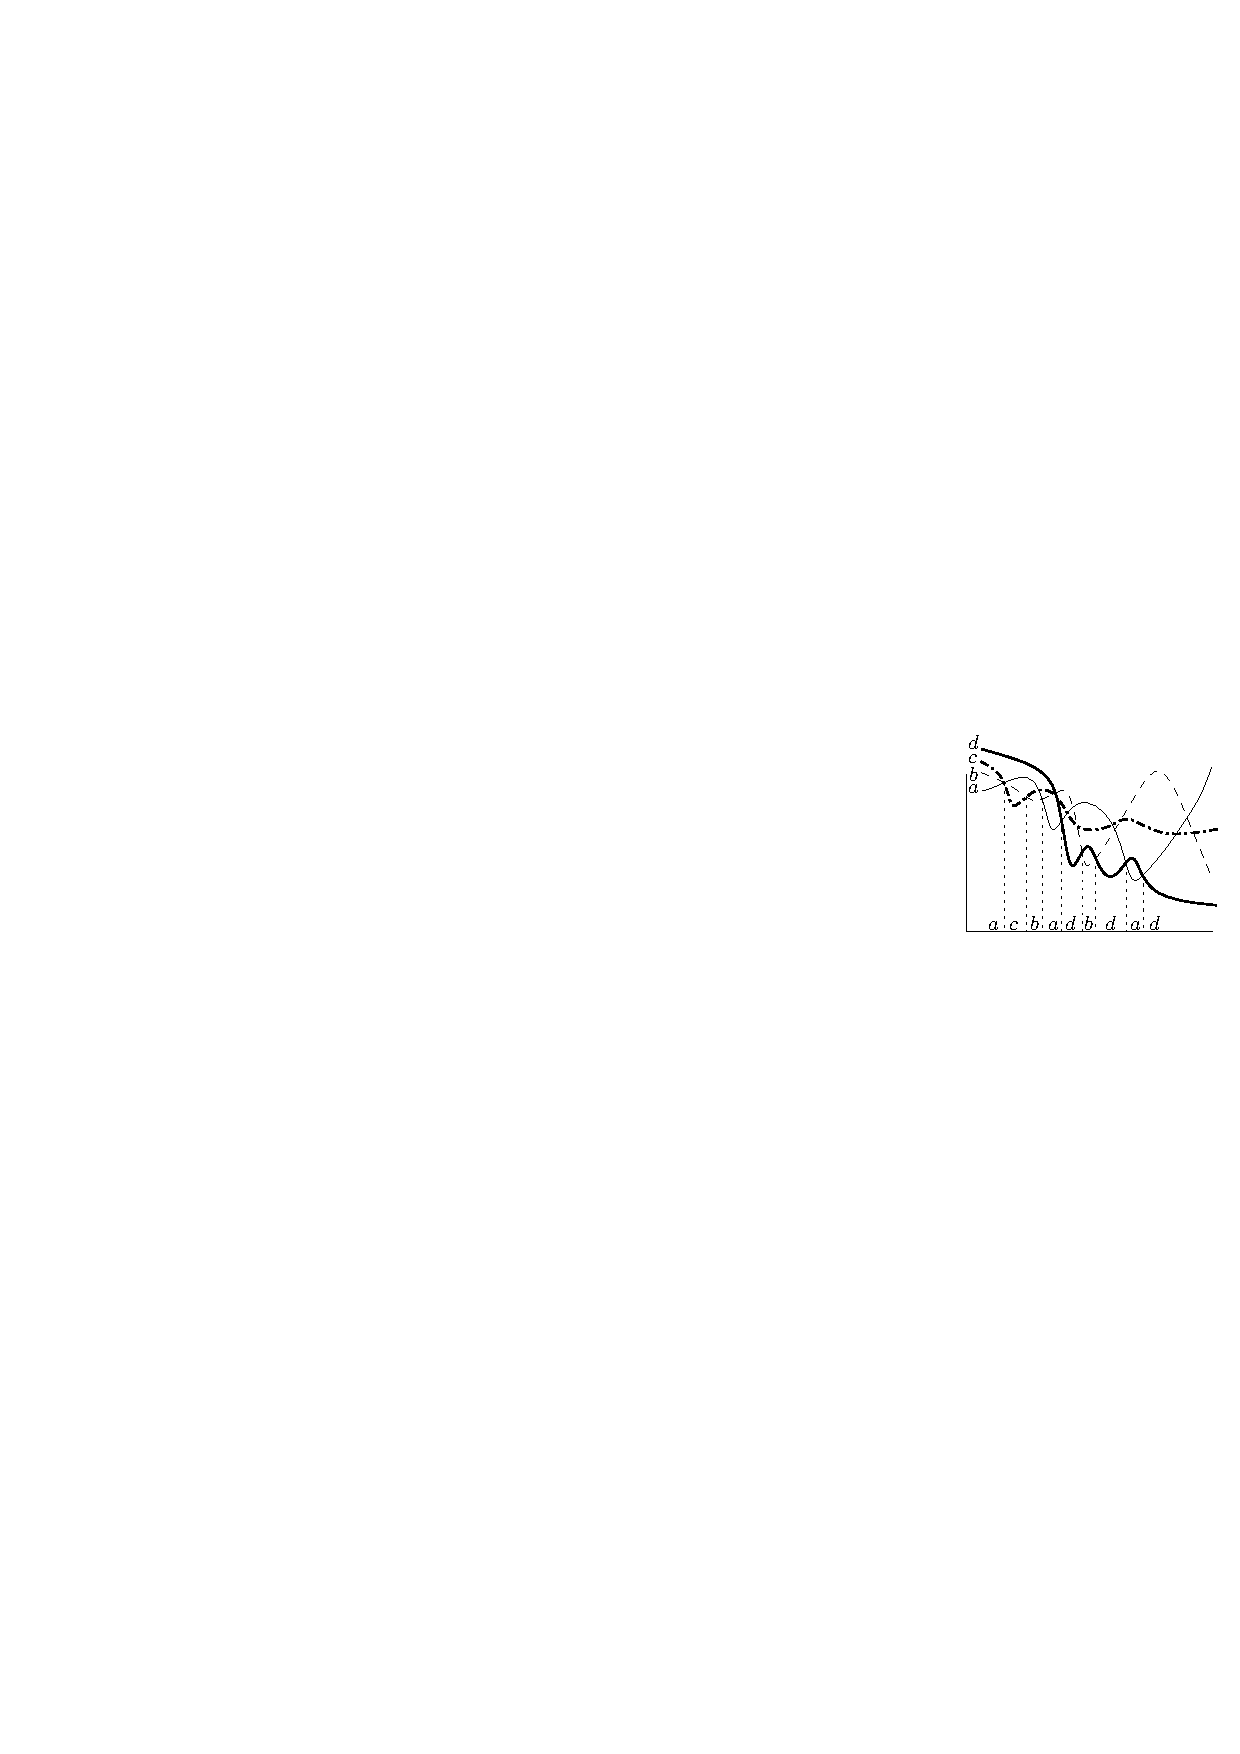
\includegraphics[width=0.5\textwidth]{DSsequence}
\end{center}
\caption{پوشش پایینی یک مجموعه از توابع متناظر با دنباله‌ای از نمادها}
\label{fig-DSsequence}
\end{figure}
اگر $\cal F$ مجموعه‌ای از $n$ تابع چندجمله‌ای با درجه‌ی $s$ باشد. با توجه به این‌که هر دو تابع چندجمله‌ای از درجه‌ی $s$ حداکثر در $s$ نقطه با یکدیگر برخورد می‌کنند (این بدان معنی است که حداکثر $s$ تناوب از هر دو تابع مجزا از $\cal F$  در $\Gamma(\cal F)$ وجود خواهد داشت) و نیز وجود دو تابع یکسان مجاور به هم در $\Gamma(\cal F)$ هم امکان ندارد، به‌راحتی می‌توان نتیجه گرفت که $\Gamma(\cal F)$ متناظر با یک $(n, s)$ دنباله‌ی داونپورت-شینزل است و پیچیدگی آن نیز، برابر با طول دنباله‌ی داونپورت-شینزل متناظر با آن خواهد شد. شکل \ref{fig-DSsequence} را ببینید. پس می‌توان گفت که پیچیدگی $\Gamma(\cal F)$ از مرتبه‌ی $O(\lambda_{s}(n))$ است. تمام نتایج به‌طور مشابه برای پیچیدگی پوشش بالایی نیز برقرار است. اگر دامنه‌ی تعریف $\Gamma(\cal F)$ در نظر گرفته شود و هر تابع چندجمله‌ای از $\cal F$  روی قسمتی از این دامنه (یک بازه مشخص از دامنه) تعریف شود، یعنی نمودار هر تابع تکه‌ای از نمودار آن تابع با دامنه نامحدود باشد، آنگاه پیچیدگی $ \Gamma(\cal F)$ برابر $O(\lambda_{s+2}(n))$ می‌شود \cite{sp-dssga-95}.
برای یک ثابت $s\geq 3$، $\lambda_{s}(n)$ یک تابع ابرخطی است اما خیلی آهسته رشد می‌کند. در ادامه قضیه‌ای بیان می‌شود که فرمول‌های مربوط به محاسبه  $\lambda_{s}(n)$ را بیان می‌کند. تابع $\alpha(n)$  به معکوس تابع آکرمان\LTRfootnote{Ackermann function} اشاره می‌کند \cite{sp-dssga-95}.


از آن جایی که $\alpha(n)$ تابعی است که بی‌نهایت آهسته رشد می‌کند (تقریبا برای مقادیر عملی و منطقاً بزرگ $n$ مقدار ثابت است)، بنابراین برای یک مقدار ثابت $s$، $\lambda_{s}(n)$ تقریبا خطی از $n$  است.   
%%%%%%%%%%%%%%%%%%%%%
 %%%%%%%%%%%%%%%%%%%
\section{پوشش‌های هندسی روی مجموعه نقاط}\label{sec-t-spann}
\subsection{شبکه‌های هندسی}
مجموعه‌ی $P$ شامل $n$ نقطه در فضای $\mathbb{R}^d$ را درنظر بگیرید، یک \textbf{شبکه‌ی متصل‌کننده‌ی نقاط} $P$\LTRfootnote{A network connecting the points of P}، یک گراف ${\cal G} = (P, E)$ با مجموعه رأس‌های $P$ و مجموعه یال‌های $E \subseteq P\times P$  است، به‌طوری‌که هر دو نقطه‌ی $p, q \in P$ با یک مسیر در $\cal G$ به‌هم متصل می‌شوند. یک \textbf{شبکه‌ی هندسی}\LTRfootnote{Geometric network} یا یک \textbf{گراف اقلیدسی}\LTRfootnote{Euclidean graph}، یک گراف وزن‌دار ${\cal G}$ است که رأس‌ها متناظر با نقاط در فضای اقلیدسی و وزن روی یال‌ها متناظر با فاصله‌‌ی اقلیدسی بین نقاط انتهایی آن یال است. شبکه‌های هندسی در واقع تعداد زیادی از شبکه‌های حقیقی موجود، مانند شبکه راه‌ها، شبکه مخابرات و غیره را مدل می‌کنند.
%\nocite{ns-gsn-07}

برای طراحی یک شبکه برای مجموعه‌ی مشخصی از نقاط، چندین معیار کیفی در نظر گرفته می‌شود. در زیر تعدادی از مهم‌ترین معیارهای کیفی برای ارزیابی شبکه‌های هندسی بیان شده است.
 \begin{enumerate}
\item
\textbf{اندازه}\LTRfootnote{Size}، به‌عنوان تعداد یال‌های شبکه تعریف می‌شود. در حالت کلی ترجیح داده می‌شود که شبکه‌ها تا جای ممکن اندازه‌ی کوچکی (خطی از تعداد نقاط) داشته باشند. 
\item
\textbf{وزن}\LTRfootnote{Weight}، به‌عنوان مجموع وزن یال‌های شبکه تعریف می‌شود. ازآن‌جایی‌که هر شبکه باید تمام نقاط را به‌هم وصل کند، درنتیجه وزن آن از پایین با وزن درخت پوشای کمینه کران‌دار می‌شود. وزن یک معیار خوب برای سنجش هزینه‌ی ساخت شبکه است. بنابراین، اغلب شبکه‌هایی با وزن کم مورد نظر هستند.
\item
\textbf{ضریب کشش}\LTRfootnote{Stretch factor}یا \textbf{تاخیر}\LTRfootnote{Dilation}  برای دو نقطه‌ی داده شده، برابر با نسبت کوتاه‌ترین مسیر (مسیر با وزن مینیمم) بین دو نقطه در شبکه، به فاصله‌ی آن دو نقطه بر اساس متر تعریف شده برای آن شبکه است (مثلاً این فاصله در متر اقلیدسی خط مستقیم متصل کننده‌ی دو نقطه است). ضریب کشش یک شبکه به‌عنوان بیش‌ترین ضریب کشش برای هر جفت از نقاط مجزا در شبکه تعریف می‌شود. در بسیاری از موارد، نیاز است که ضریب کشش شبکه با یک ثابت کوچک محدود شود (که حداقل باید یک باشد). شبکه‌ها با ضریب کشش حداکثر $t$، $t$-پوشش‌ها\LTRfootnote{t-Spanners} نامیده می‌شوند.
\item
\textbf{درجه}\LTRfootnote{Degree}،  بیش‌ترین تعداد یال‌های مجاور به هر نقطه در شبکه می‌باشد و اغلب نیاز است که با یک ثابت کوچک محدود شود. درجه‌ی محدود یک شبکه، به اندازه‌ی کوچک آن شبکه اشاره می‌کند، اما برعکس این مطلب لزوماً درست نیست.
\end{enumerate}
در حالت کلی، در زمان طراحی یک شبکه، آن‌چه که اهمیت زیادی دارد، اعمال ترکیبی از این معیارهای کیفی بر روی شبکه است و در زمان تحلیل شبکه نیز ویژگی‌های شبکه، نسبت به این معیارها سنجیده می‌شود. یکی از مسائل مهم در این زمینه، مطالعه‌ی شبکه‌هایی با ضریب کشش کم است (در ترکیب با دیگر ویژگی‌ها). ازجمله، در بسیاری از کاربردها مانند شبکه‌ی راه‌ها لازم است یک ارتباط سریع (مستقیم) بین هر جفت از نقاط در $P$ برقرار باشد (یعنی شبکه یک گراف کامل باشد) ولی این نیاز به خاطر هزینه‌های بالا، قابل اجرا شدن نیست. بنابراین نیاز به مطالعه‌ی شبکه‌هایی با ضریب کشش کم، منجر به شکل‌گیری مفهوم پوشش‌های هندسی می‌شود. این پوشش‌ها در واقع یک ساختار برای شبکه‌ها، زمانی که ارتباطات کوتاه بین نقاط اهمیت دارند را فراهم می‌کنند.
%%%%%%%%%%%%%%%%%%%%%%%%%%%%%%%%
\subsection{$t$-پوشش‌های هندسی}
 \begin{definition}
\label{def-t-spanner}
مجموعه‌ی $P$ شامل $n$ نقطه در فضای $\mathbb{R}^d$ و $t \geq 1$ را یک عدد حقیقی درنظر بگیرید. یک $t$-\textbf{پوشش}\LTRfootnote{t-spanner} برای $P$، یک گراف بدون ‌جهت $\cal G$ با مجموعه رأس‌های $P$  است، به‌طوری‌که کوتاه‌ترین مسیر بین هر دو نقطه‌ی $p$ و $q$ از $P$،  در $\cal G$ که با نماد $d_{\cal G}(p, q)$ نشان داده می‌شود، این شرط را داشته باشد:
$$d_{\cal G}(p, q) \leq t \cdot ||pq||.$$ هر مسیری که این شرط را برآورده سازد یک $t$-\textbf{مسیر}\LTRfootnote{t-path} بین $p$ و $q$ نامیده می‌شود.
\end{definition}
 برای هر عدد حقیقی $t^{'}$ که $t^{'} > t$ است، اگر $\cal G$ یک $t$-پوشش برای مجموعه نقاط $P$  باشد، بدیهی است که $\cal G$ یک $t^{'}$-پوشش نیز برای $P$ است. این، منجر به تعریف زیر می‌شود:
 \begin{definition}[\textbf{ضریب کشش}]
\label{def-strtch-factor}
مجموعه‌ی $P$ شامل $n$ نقطه در فضای $\mathbb{R}^d$ و $\cal G$ را یک گراف اقلیدسی با مجموعه رأس‌های $P$ درنظر بگیرید. ضریب کشش $\cal G$، کوچک‌ترین عدد حقیقی $t$ است به‌طوری‌که $\cal G$ یک $t$-پوشش از $P$ باشد.
\end{definition}
گراف کامل یک 1-پوشش است، اما تعداد مربعی یال دارد. درحقیقت، اگر فرض شود که هیچ سه نقطه‌ای از $P$  روی یک خط قرار ندارند، سپس گراف کامل تنها 1-پوشش برای $P$ است. بنابراین، در حالت کلی $t$-پوشش‌ها برای $t$ های بزرگ‌تر از یک بررسی می‌شوند. اما از آن‌جایی که در بسیاری از کاربردها، پوشش‌هایی با ارتباطات سریع (ضریب کشش کم) مورد نیاز هستند. بنابراین پوشش‌هایی با ضریب کشش نزدیک به یک، مورد مطالعه قرار می‌گیرند، یعنی $t = 1 + \varepsilon$،  برای مقادیر $\varepsilon$ مثبت و کوچک ($0 < \varepsilon < 1$). به این ترتیب، می‌توان با انتخاب مقادیر خیلی کوچک برای $\varepsilon$، مقدار $t$ را به یک نزدیک کرد، یعنی $t$-پوشش را به یک $1$-پوشش (گراف کامل) نزدیک کرد.
 %%%%%%%%%%%%%%%%%%%%%%%%%

 \section{ یک پوشش هندسی وابسته به حرکت در صفحه}
در این فصل یک $1 + \varepsilon$-پوشش ساده با اندازه‌ی خطی، برای یک مجموعه از $n$ نقطه در صفحه معرفی می‌شود. این پوشش زمانی‌که نقاط آن حرکت می‌کنند، می‌تواند به‌صورتی کارا نگهداری شود. فرض می‌شود که مسیر حرکت نقاط با توابع شبه‌جبری از درجه‌ی حداکثر $s$ توصیف می‌شوند (بخش \ref{sec-model-motion} را ببینید). لازم به ذکر است که مطالب این فصل بر اساس مقاله‌ی آبام\LTRfootnote{Abam} و همکارانش \cite{abg-seks-10} تنظیم شده است. \section{کارهای مرتبط}
یک $1 + \varepsilon$-پوشش را درنظر بگیرید. برای جزئیات بیش‌تر در مورد پوشش‌ها می‌توانید بخش \ref{sec-t-spann} را ببینید. هنگامی که نقاط پوشش دارای حرکت پیوسته‌ای از زمان باشند، پوشش به‌طور پیوسته از زمان تغییر می‌کند، اما تنها در لحظه‌های مشخصی نیاز به به‌روزرسانی خواهد داشت، تا همچنان در تمام زمان‌ها یک $1 + \varepsilon$-پوشش باقی بماند. در فصل 2 بیان شد که این لحظات رویداد نامیده می‌شوند. از آن‌جایی که کارایی و پاسخ‌گویی، از مهم‌ترین معیارها برای ارزیابی کیفیت ساختارهای وابسته به حرکت هستند، هدف، طراحی پوششی است که تعداد رویدادها و نیز زمان پاسخ‌گویی آن، کم باشد. همان‌طورکه در فصل 2 بیان شد، در حالت ایده‌ال، تعداد رویدادها باید نزدیک به کم‌ترین تعداد رویدادهایی که برای نگهداری ساختار لازم است باشد. برای پوشش‌ها، این بدین معنی است که تعداد رویدادها باید $O(n^{2})$ باشد؛ زیرا مجموعه‌های $n$ تایی از نقاط که به‌صورت خطی در صفحه حرکت می‌کنند وجود دارند، که برای هر $1 + \varepsilon$-پوشش باید $\Omega(n^{2}/(1 + \varepsilon)^{2})$ رویداد پردازش شود.
% \cite{ggn-dsa-06}. 
زمان پاسخ‌گویی نیز در حالت ایده‌ال باید چندلگاریتمی باشد.

\subsection{تحلیل ضریب کشش و اندازه‌ی پوشش}  \label{subsec-span-ratio}
در این زیربخش ثابت خواهد ‌شد که اگر زاویه‌های $\phi$ و $\varphi$ به‌گونه‌ای انتخاب شوند که شرط‌های 
%\begin{latin}
\begin{equation}\label{eq-rd-first}
(\cos \phi - \sin \phi) \geq 1/(1 + \varepsilon) 
\end{equation} 
%\end{latin}
و
 \begin{equation}\label{eq-rd-sec}(\sin(\phi/2)/\sin(\varphi/2)) \geq 1 + 2/\varepsilon \end{equation}
 برقرار باشند، آنگاه ${\cal DDS}(P)$ یک $1 + \varepsilon$-پوشش برای مجموعه نقاط $P$ خواهد بود. این شرط‌ها می‌توانند با تنظیم زوایای $\phi$ و $\varphi$ به‌صورت  $ \phi = \arcsin \frac{\varepsilon}{2(1+\varepsilon)}$ و $ \varphi = 2\arcsin \frac{\varepsilon^{2}}{4(1+\varepsilon)(2+\varepsilon)}$  به‌دست آیند. همواره فرض می‌شود که $\varphi <\phi$.  
\begin{observation}
\label{obsr-phi}
اگر $ \phi = \arcsin \frac{\varepsilon}{2(1+\varepsilon)}$ برقرار باشد آنگاه $0 < \phi < \dfrac{\pi}{6}$.
\end{observation}
\begin{proof}
از آن‌جایی‌که، $\dfrac{\varepsilon}{2(1+\varepsilon)} < \dfrac{1}{2}$  و تابع $\arcsin$ در بازه $ (0, \pi/2)$ یک تابع صعودی است، بنابراین،
 $$0 < \phi = \arcsin \frac{\varepsilon}{2(1+\varepsilon)} < \arcsin \frac{1}{2} = \dfrac{\pi}{6}.$$
\end{proof}
\begin{observation}
\label{obsr-angles}
با انتخاب $ \phi = \arcsin \frac{\varepsilon}{2(1+\varepsilon)}$ و $\varphi = 2\arcsin \frac{\varepsilon^{2}}{4(1+\varepsilon)(2+\varepsilon)}$ دو شرط \ref{eq-rd-first} و \ref{eq-rd-sec} برقرار است.
\end{observation}
مشتق\index{مشتق} تابع $f$، تابعی است که با علامت $f'$ نشان داده می‌شود و مقدار آن در هر عدد $x$ واقع در دامنهٔ $f$
به صورت 
\begin{align}\label{bderi1}
f'(x)=\lim_{\Delta x\rightarrow 0}\dfrac{f(x+\Delta x) - f(x)}{\Delta x}
\end{align}
\ysymbol{$f'(x)$}{مشتق تابع $f$ در نقطهٔ $x$}
تعریف می‌شود؛ به شرطی که حد فوق وجود داشته باشد.

اگر $f$ روی بازهٔ $[a,b]$ هموار باشد، طول منحنی $y=f(x)$ از $a$ تا $b$ برابر است با
\begin{align}\label{10eq6}
L=\int_a^b \sqrt{1+\Big(\dfrac{dy}{dx}\Big)^2}dx=\int_a^b \sqrt{1+(f'(x))^2}dx.
\ysymbol{$L$}{طول منحنی}
\end{align}

اگر تابع $f$ در $x_1$ تعریف شده باشد، آنگاه مشتق راست $f$ در $x_1$ با $f'_{+}(x_1)$ 
\ysymbol{$f'_{+}(x)$}{مشتق راست  $f$ در نقطهٔ $x$}
نشان داده می‌شود و به صورت 
\begin{align}
f'_{+}(x_1)=\lim_{\Delta x\rightarrow 0^{+}}\dfrac{f(x_1+\Delta x) - f(x_1)}{\Delta x}
\end{align}
و یا به عبارت دیگر،
تعریف می‌شود؛ به شرطی که این حدود موجود باشند.

\begin{example}
نمونه مثال
\end{example}
\begin{proposition}
نمونه گزاره
\end{proposition}
\begin{corollary}
نمونه نتیجه
\end{corollary}

\begin{remark}
نمونه ملاحظه
\end{remark}


!
داخل فایل
\LRE{\verb!yazd-thesis.tex!}
و بعد از دستور
\verb!\chapter{راهنمای استفاده از کلاس \lr{yazd-thesis}}
\section{مقدمه}
حروف‌چینی پایان‌نامه یا رساله یکی از موارد پرکاربرد استفاده از زی‌پرشین است. از طرفی، یک  پایان‌نامه یا رساله،  احتیاج به تنظیمات زیادی از نظر صفحه‌آرایی  دارد که ممکن است برای
یک کاربر مبتدی، مشکل باشد. به همین خاطر، برای راحتی کار کاربر، کلاس حاضر با نام 
 \LRE{\verb!yazd-thesis!}
 برای حروف‌چینی پروژه‌ها، پایان‌نامه‌ها و رساله‌های دانشگاه یزد با استفاده از نرم‌افزار زی‌پرشین،  آماده شده است. این فایل به 
گونه‌ای طراحی شده است که کلیه خواسته‌های مورد نیاز  مدیریت تحصیلات تکمیلی دانشگاه یزد را برآورده می‌کند. همچنین حروف‌چینی بسیاری
از قسمت‌های آن، به طور خودکار انجام می‌شود.

کلیه فایل‌های لازم برای حروف‌چینی با کلاس گفته شده، داخل پوشه‌ای به نام
 \LRE{\verb!yazd-thesis!}
  قرار داده شده است. توجه داشته باشید که برای استفاده از این کلاس باید فونت
 \verb!Yas!
    روی سیستم شما نصب شده باشد.
\section{این همه فایل؟!}\label{sec2}
از آنجایی که یک پایان‌نامه یا رساله، یک نوشته بلند محسوب می‌شود، لذا اگر همه تنظیمات و مطالب پایان‌نامه را داخل یک فایل قرار بدهیم، باعث شلوغی
و سردرگمی می‌شود. به همین خاطر، قسمت‌های مختلف پایان‌نامه یا رساله  داخل فایل‌های جداگانه قرار گرفته است. مثلاً تنظیمات  کلاس داخل فایل
\LRE{\verb!yazd-thesis.cls!}، 
قسمت مشخصات فارسی پایان‌نامه داخل 
\LRE{\verb!fainfo.tex!}،
مطالب فصل اول، داخل 
\verb!chapter1!
و ... قرار داده شده است. نکته مهمی که در اینجا وجود دارد این است که از بین این  فایل‌ها، فقط فایل 
\LRE{\verb!yazd-thesis.tex!}
قابل اجرا است. یعنی بعد از تغییر فایل‌های دیگر، برای دیدن نتیجه تغییرات، باید این فایل را اجرا کرد. بقیه فایل‌ها به این فایل، کمک می‌کنند تا بتوانیم خروجی کار را ببینیم. اگر به فایل 
\LRE{\verb!yazd-thesis.tex!}
دقت کنید، متوجه می‌شوید که قسمت‌های مختلف پایان‌نامه، توسط دستورهایی مانند 
\verb!input!
و
\verb!include!
به فایل اصلی، یعنی 
\LRE{\verb!yazd-thesis.tex!}
معرفی شده‌اند. بنابراین، فایلی که همیشه با آن سروکار داریم، فایل 
\LRE{\verb!yazd-thesis.tex!}
است.
در این فایل، فرض شده است که پایان‌نامه یا رساله، از ۳ فصل و یک پیوست، تشکیل شده است. با این حال، اگر
  پایان‌نامه یا رساله، بیشتر از ۳ فصل و یک پیوست است، باید خودتان فصل‌های بیشتر را به این فایل، اضافه کنید. این کار، بسیار ساده است. فرض کنید بخواهید یک فصل دیگر هم به پایان‌نامه، اضافه کنید. برای این کار، کافی است یک فایل با نام 
\verb!chapter4!
و با پسوند 
\verb!.tex!
بسازید و آن را داخل پوشه 
\LRE{\verb!yazd-thesis!}
قرار دهید و سپس این فایل را با دستور 
\verb!\chapter{ نمونه‌ای از یک فصل}
\section{مدل‌های حرکت}\label{sec-model-motion}
بسته به کاربرد، حرکت مجموعه نقاط در فضای دلخواه از راه‌های مختلف نمایش داده می‌شود. حرکت می‌تواند به صورت صریح با توابع چندجمله‌ای، به صورت ضمنی با معادلات دیفرانسیلی، یا به صورت آماری با مدل‌های احتمالی نمایش داده شود. همان‌طورکه بعداً دیده خواهد شد، در مسائل وابسته به حرکت که نقاط مسئله به‌طور پیوسته در حال حرکت هستند، لازم است تا وضعیت نقاط در هر زمان با مجموعه‌ای از شرط‌های جبری مشخص شود. علاوه بر این نیاز است تا مسیر حرکت نقاط به‌گونه‌ای تعریف شود که تعداد دفعاتی که یک شرط جبری ممکن است نامعتبر ‌شود ثابت باشد. بدین منظور در این پایان‌نامه، فرض می‌شود که مسیر حرکت نقاط در صفحه به صورت  \textbf{حرکت‌های شبه‌جبری}\LTRfootnote{Pseudo algebraic motions} است. برای تعریف این نوع حرکت‌ها لازم است توابع شبه‌جبری تعریف شوند، که از تعریف زانگ\LTRfootnote{Zhang} مطرح شده در
 %\cite{z-kmps-00} 
 استفاده می‌شود. 

\begin{definition}\label{def-psdo-algb-func}
توابع پیوسته‌ی یک متغیره‌ی $f_{1}(x), f_{2}(x), ... , f_{m}(x)$، توابع شبه‌جبری از درجه‌ی حداکثر $s$ هستند، هرگاه برای هر تابع چندجمله‌ای $m$ متغیره‌ی $g$  از درجه‌ی $s_{1}$،  تابع  $$h(x) = g(f_{1}(x), f_{2}(x), ... , f_{m}(x))$$  متحد صفر باشد یا حداکثر $s \times s_{1}$  ریشه داشته باشد.
 \end{definition}
  برای نمونه، توابع چندجمله‌ای یا منطقی با درجه‌ی ثابت توابع شبه‌جبری هستند. یک مجموعه از نقاط دارای حرکت‌های شبه‌جبری از زمان هستند هرگاه مسیر حرکت آن‌ها با توابع شبه‌جبری از زمان توصیف شود. در ادامه، تعریف \ref{def-psdo-algb-func} با شرح یک مثال توضیح داده می‌شود. 
 
مسئله‌ی یک بعدی زیر که ترتیب $n$ نقطه‌ی در حال حرکت روی محور $x$ ها را گزارش می‌کند، درنظر بگیرید. هر نقطه‌ی $p_{i}$  دارای مسیر حرکت پیوسته‌ای از زمان است که با $f_{i}(t)$  نشان داده می‌شود و $t$ به زمان اشاره می‌کند. مقدار هر نقطه‌ی $p_{i}$  در زمان $t$، یعنی مولفه‌ی $x$ نقطه، با $v_{i}(t)$ نشان داده می‌شود. فرض کنید مجموعه توابع حرکت نقاط، یعنی $f_{1}(t), f_{2}(t), ... ، f_{n}(t)$،  توابع شبه‌جبری از درجه‌ی $s$ باشند و شرط‌های جبری برای تعیین موقعیت نقاط متحرک از نوع مقایسه تعریف شوند. اگر برای نشان دادن ترتیب هر دو نقطه‌ی متوالی $p_{i}$ و $p_{j}$ روی محور $x$ در زمان $t$، به‌طوری‌که $ v_{j}(t) > v_{i}(t)$ باشد، از شرط جبری $ v_{j}(t) - v_{i}(t) > 0$  استفاده شود، آنگاه با توجه به تعریف \mbox{\ref{def-psdo-algb-func}}، می‌توان تابع دو متغیره‌ی خطی $g(f_{j}, f_{i})(t) =  f_{j}(t) - f_{i}(t)$ (که طبق تعریف دارای $s_{1} = 1$ و $m = 2$ است)، را به عنوان تابع $h(t)$ درنظر گرفت و به این نتیجه رسید که تابع $h(t) = g(f_{j}, f_{i})(t)$ یا متحد صفر است یا دارای حداکثر $s \times 1$  ریشه است. این بدان معنی است که شرط جبری $ v_{j}(t) - v_{i}(t) > 0$ با گذشت زمان حداکثر به تعداد $s$ بار صفر می‌شود و متعاقباً تغییر علامت می‌دهد (تغییر ترتیب نقاط).
 
در تحلیل مسائلی که بعداً مطرح خواهند شد، بسیار اهمیت دارد که تعداد دفعاتی که شرط جبری مربوط به یک نقطه با گذشت زمان صفر می‌شود ثابت باشد. از آن‌جایی که در بیش‌تر مسائل شرط‌های جبری که برای تعیین وضعیت نقاط معرفی می‌شوند، چندجمله‌ای‌هایی از درجه‌ی کم، تعریف شده روی یک تعداد ثابت از نقاط هستند، فرض شبه‌جبری بودن حرکت نقاط کافی است تا برقراری این موضوع را تضمین کند. برای نمونه، در مثال بالا شرط‌های جبری (مقایسه‌ی دو مقدار) از درجه‌ی یک و تعریف شده روی دو نقطه هستند، بنابراین با فرض شبه‌جبری بودن حرکت نقاط، شرط جبری مربوط به یک نقطه همان تابع $g$ مطرح شده در تعریف \ref{def-psdo-algb-func} می‌شود که حداکثر به تعداد $s \times 1$  بار صفر خواهد شد ( $s$ یک عدد ثابت که درجه‌ی توابع شبه‌جبری حرکت را نشان می‌دهد). 

 \section{دنباله‌ی داونپورت-شینزل}\label{sec-DS-sequence}
 \begin{definition}
\label{def-DS-sequ}
یک $(n, s)$ دنباله‌ی داونپورت-شینزل\LTRfootnote{Davenport-Schinzel sequence}، که $n$ و $s$ اعداد صحیح مثبت هستند، یک دنباله‌ی ساخته شده از $n$ نماد با این خواص است که هیچ دو نماد مجاور در دنباله یکسان نیستند و این‌که برای هر دو نماد مجزای $a$ و $b$  حداکثر $s$  تناوب از آن‌ها در دنباله وجود دارد.
 \end{definition}
در تعریف بالا، منظور از تناوب $a$ و $b$ این است که نماد $b$ بعد از نماد $a$ و نماد $a$ بعد از نماد $b$ در دنباله ظاهر شود، ولی نه الزاماً مجاور به هم (کنار هم). مثلاً دنباله‌ی زیر، تشکیل شده از نمادهای $a, b, c, d$ را در نظر بگیرید: $$\underline{a}c\underline{b}dbc\underline{a}cd
\underline{b}\underline{a}dcdcadc\underline{b}$$ تعداد تناوب‌های $a$ و $b$ در دنباله، یعنی مجموع تعداد دفعاتی که $b$ بعد از $a$  و $a$ بعد از $b$ در دنباله ظاهر شده است، برابر با 5 است. با توجه به تعریف $(n, s)$ دنباله‌ی داونپورت-شینزل، می‌توان دریافت که با یک $n$ و $s$ معلوم (داده شده)، بسته به مقدارهای $n$ و $s$،  دنباله‌‌های داونپورت-شینزل متعددی می‌توان یافت، اما همگی دارای طول‌های متناهی هستند؛ زیرا با توجه به تعریف، امکان وجود دو نماد مجاور یکسان در دنباله نیست و نیز تعداد تناوب‌های هر دو نماد مجزا در دنباله به تعداد حداکثر $s$ محدود شده است. مثلاً برای $n = 3$ و $s = 2$ و نمادهای $a, b, c$،  طول  $(3, 2)$ دنباله‌های داونپورت-شینزل ممکن، حداکثر 5 است؛ زیرا هر دنباله با طول 6 یا بیش‌تر متشکل از این نمادها، یا حداقل برای یک جفت نماد مجزا دارای بیش از 2 تناوب خواهد بود یا دو نماد مجاور یکسان خواهد داشت و در نتیجه، شرایط تعریف یک $(3, 2)$ دنباله‌ی داونپورت-شینزل را نخواهد داشت، به عنوان مثال دنباله‌ی $abcbab$ که 3 تناوب از $a$ و $b$ را دارد. بنابراین طول طولانی‌ترین $(n, s)$ دنباله‌ی داونپورت-شینزل قابل تعریف خواهد بود 
و با $\lambda_{s}(n)$ نشان داده می‌شود. در ادامه به بیان اهمیت و کاربرد این دنباله‌ها در تحلیل مسائلی‌ مهم در هندسه‌ی محاسباتی پرداخته می‌شود.

اگر $\rbrace$ $f_{i}$ $ \lbrace$ $\cal F =$
  یک مجموعه از توابع باشد،  \textbf{ پوشش پایینی}\LTRfootnote{Lower envelope}  برای مجموعه $\cal F$  برابر تابع $\min f_{i}(x)$ است که با  $\Gamma(\cal F)$ نشان داده می‌شود.  به طور مشابه  $\max f_{i}(x)$ به عنوان \textbf{پوشش بالایی}\LTRfootnote{Upper envelope}  تعریف می‌شود. پیچیدگی $\Gamma(\cal F)$ نیز برابر با تعداد دفعاتی که تابع موجود در $\Gamma(\cal F)$ عوض می‌شود، یعنی تعداد نقاط شکست $\Gamma(\cal F)$ تعریف می‌شود. 

\begin{figure}[h]
\begin{center}
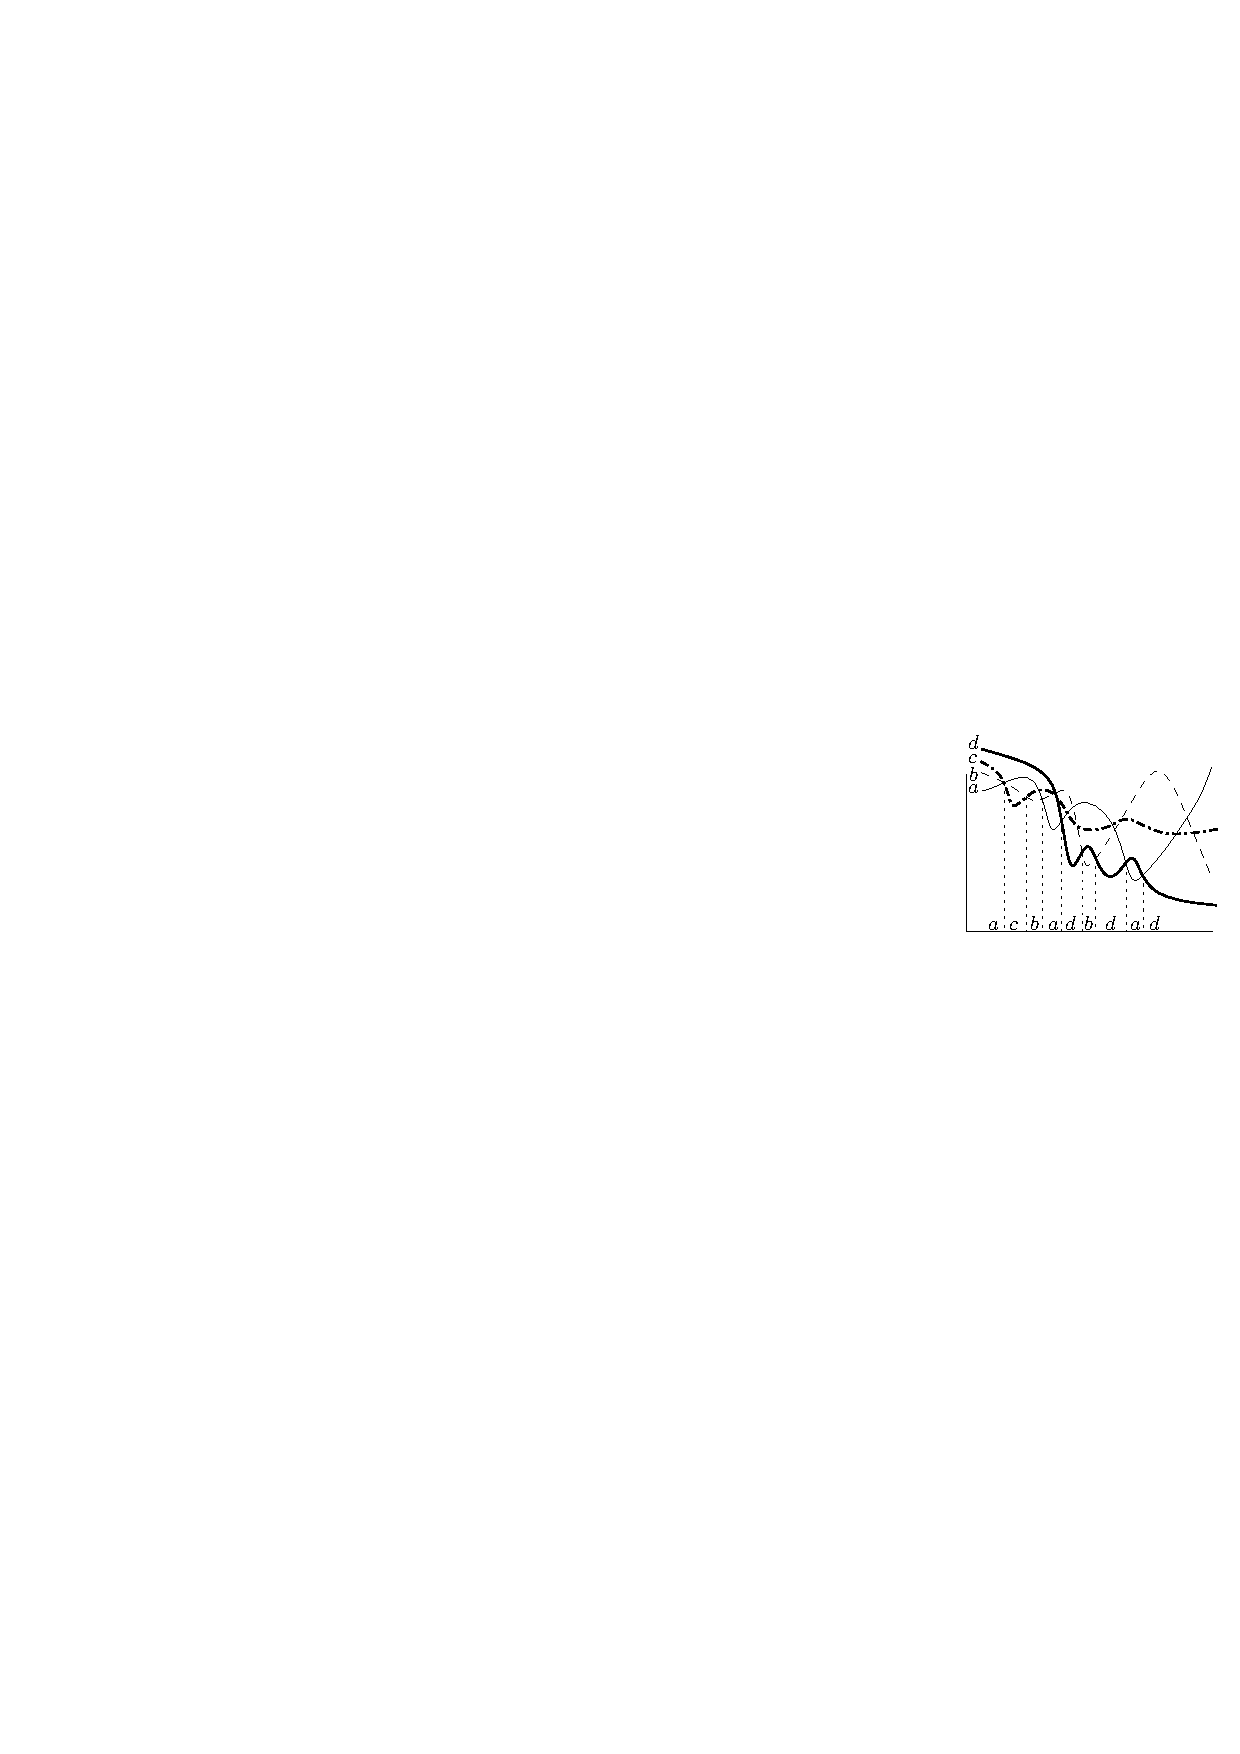
\includegraphics[width=0.5\textwidth]{DSsequence}
\end{center}
\caption{پوشش پایینی یک مجموعه از توابع متناظر با دنباله‌ای از نمادها}
\label{fig-DSsequence}
\end{figure}
اگر $\cal F$ مجموعه‌ای از $n$ تابع چندجمله‌ای با درجه‌ی $s$ باشد. با توجه به این‌که هر دو تابع چندجمله‌ای از درجه‌ی $s$ حداکثر در $s$ نقطه با یکدیگر برخورد می‌کنند (این بدان معنی است که حداکثر $s$ تناوب از هر دو تابع مجزا از $\cal F$  در $\Gamma(\cal F)$ وجود خواهد داشت) و نیز وجود دو تابع یکسان مجاور به هم در $\Gamma(\cal F)$ هم امکان ندارد، به‌راحتی می‌توان نتیجه گرفت که $\Gamma(\cal F)$ متناظر با یک $(n, s)$ دنباله‌ی داونپورت-شینزل است و پیچیدگی آن نیز، برابر با طول دنباله‌ی داونپورت-شینزل متناظر با آن خواهد شد. شکل \ref{fig-DSsequence} را ببینید. پس می‌توان گفت که پیچیدگی $\Gamma(\cal F)$ از مرتبه‌ی $O(\lambda_{s}(n))$ است. تمام نتایج به‌طور مشابه برای پیچیدگی پوشش بالایی نیز برقرار است. اگر دامنه‌ی تعریف $\Gamma(\cal F)$ در نظر گرفته شود و هر تابع چندجمله‌ای از $\cal F$  روی قسمتی از این دامنه (یک بازه مشخص از دامنه) تعریف شود، یعنی نمودار هر تابع تکه‌ای از نمودار آن تابع با دامنه نامحدود باشد، آنگاه پیچیدگی $ \Gamma(\cal F)$ برابر $O(\lambda_{s+2}(n))$ می‌شود \cite{sp-dssga-95}.
برای یک ثابت $s\geq 3$، $\lambda_{s}(n)$ یک تابع ابرخطی است اما خیلی آهسته رشد می‌کند. در ادامه قضیه‌ای بیان می‌شود که فرمول‌های مربوط به محاسبه  $\lambda_{s}(n)$ را بیان می‌کند. تابع $\alpha(n)$  به معکوس تابع آکرمان\LTRfootnote{Ackermann function} اشاره می‌کند \cite{sp-dssga-95}.


از آن جایی که $\alpha(n)$ تابعی است که بی‌نهایت آهسته رشد می‌کند (تقریبا برای مقادیر عملی و منطقاً بزرگ $n$ مقدار ثابت است)، بنابراین برای یک مقدار ثابت $s$، $\lambda_{s}(n)$ تقریبا خطی از $n$  است.   
%%%%%%%%%%%%%%%%%%%%%
 %%%%%%%%%%%%%%%%%%%
\section{پوشش‌های هندسی روی مجموعه نقاط}\label{sec-t-spann}
\subsection{شبکه‌های هندسی}
مجموعه‌ی $P$ شامل $n$ نقطه در فضای $\mathbb{R}^d$ را درنظر بگیرید، یک \textbf{شبکه‌ی متصل‌کننده‌ی نقاط} $P$\LTRfootnote{A network connecting the points of P}، یک گراف ${\cal G} = (P, E)$ با مجموعه رأس‌های $P$ و مجموعه یال‌های $E \subseteq P\times P$  است، به‌طوری‌که هر دو نقطه‌ی $p, q \in P$ با یک مسیر در $\cal G$ به‌هم متصل می‌شوند. یک \textbf{شبکه‌ی هندسی}\LTRfootnote{Geometric network} یا یک \textbf{گراف اقلیدسی}\LTRfootnote{Euclidean graph}، یک گراف وزن‌دار ${\cal G}$ است که رأس‌ها متناظر با نقاط در فضای اقلیدسی و وزن روی یال‌ها متناظر با فاصله‌‌ی اقلیدسی بین نقاط انتهایی آن یال است. شبکه‌های هندسی در واقع تعداد زیادی از شبکه‌های حقیقی موجود، مانند شبکه راه‌ها، شبکه مخابرات و غیره را مدل می‌کنند.
%\nocite{ns-gsn-07}

برای طراحی یک شبکه برای مجموعه‌ی مشخصی از نقاط، چندین معیار کیفی در نظر گرفته می‌شود. در زیر تعدادی از مهم‌ترین معیارهای کیفی برای ارزیابی شبکه‌های هندسی بیان شده است.
 \begin{enumerate}
\item
\textbf{اندازه}\LTRfootnote{Size}، به‌عنوان تعداد یال‌های شبکه تعریف می‌شود. در حالت کلی ترجیح داده می‌شود که شبکه‌ها تا جای ممکن اندازه‌ی کوچکی (خطی از تعداد نقاط) داشته باشند. 
\item
\textbf{وزن}\LTRfootnote{Weight}، به‌عنوان مجموع وزن یال‌های شبکه تعریف می‌شود. ازآن‌جایی‌که هر شبکه باید تمام نقاط را به‌هم وصل کند، درنتیجه وزن آن از پایین با وزن درخت پوشای کمینه کران‌دار می‌شود. وزن یک معیار خوب برای سنجش هزینه‌ی ساخت شبکه است. بنابراین، اغلب شبکه‌هایی با وزن کم مورد نظر هستند.
\item
\textbf{ضریب کشش}\LTRfootnote{Stretch factor}یا \textbf{تاخیر}\LTRfootnote{Dilation}  برای دو نقطه‌ی داده شده، برابر با نسبت کوتاه‌ترین مسیر (مسیر با وزن مینیمم) بین دو نقطه در شبکه، به فاصله‌ی آن دو نقطه بر اساس متر تعریف شده برای آن شبکه است (مثلاً این فاصله در متر اقلیدسی خط مستقیم متصل کننده‌ی دو نقطه است). ضریب کشش یک شبکه به‌عنوان بیش‌ترین ضریب کشش برای هر جفت از نقاط مجزا در شبکه تعریف می‌شود. در بسیاری از موارد، نیاز است که ضریب کشش شبکه با یک ثابت کوچک محدود شود (که حداقل باید یک باشد). شبکه‌ها با ضریب کشش حداکثر $t$، $t$-پوشش‌ها\LTRfootnote{t-Spanners} نامیده می‌شوند.
\item
\textbf{درجه}\LTRfootnote{Degree}،  بیش‌ترین تعداد یال‌های مجاور به هر نقطه در شبکه می‌باشد و اغلب نیاز است که با یک ثابت کوچک محدود شود. درجه‌ی محدود یک شبکه، به اندازه‌ی کوچک آن شبکه اشاره می‌کند، اما برعکس این مطلب لزوماً درست نیست.
\end{enumerate}
در حالت کلی، در زمان طراحی یک شبکه، آن‌چه که اهمیت زیادی دارد، اعمال ترکیبی از این معیارهای کیفی بر روی شبکه است و در زمان تحلیل شبکه نیز ویژگی‌های شبکه، نسبت به این معیارها سنجیده می‌شود. یکی از مسائل مهم در این زمینه، مطالعه‌ی شبکه‌هایی با ضریب کشش کم است (در ترکیب با دیگر ویژگی‌ها). ازجمله، در بسیاری از کاربردها مانند شبکه‌ی راه‌ها لازم است یک ارتباط سریع (مستقیم) بین هر جفت از نقاط در $P$ برقرار باشد (یعنی شبکه یک گراف کامل باشد) ولی این نیاز به خاطر هزینه‌های بالا، قابل اجرا شدن نیست. بنابراین نیاز به مطالعه‌ی شبکه‌هایی با ضریب کشش کم، منجر به شکل‌گیری مفهوم پوشش‌های هندسی می‌شود. این پوشش‌ها در واقع یک ساختار برای شبکه‌ها، زمانی که ارتباطات کوتاه بین نقاط اهمیت دارند را فراهم می‌کنند.
%%%%%%%%%%%%%%%%%%%%%%%%%%%%%%%%
\subsection{$t$-پوشش‌های هندسی}
 \begin{definition}
\label{def-t-spanner}
مجموعه‌ی $P$ شامل $n$ نقطه در فضای $\mathbb{R}^d$ و $t \geq 1$ را یک عدد حقیقی درنظر بگیرید. یک $t$-\textbf{پوشش}\LTRfootnote{t-spanner} برای $P$، یک گراف بدون ‌جهت $\cal G$ با مجموعه رأس‌های $P$  است، به‌طوری‌که کوتاه‌ترین مسیر بین هر دو نقطه‌ی $p$ و $q$ از $P$،  در $\cal G$ که با نماد $d_{\cal G}(p, q)$ نشان داده می‌شود، این شرط را داشته باشد:
$$d_{\cal G}(p, q) \leq t \cdot ||pq||.$$ هر مسیری که این شرط را برآورده سازد یک $t$-\textbf{مسیر}\LTRfootnote{t-path} بین $p$ و $q$ نامیده می‌شود.
\end{definition}
 برای هر عدد حقیقی $t^{'}$ که $t^{'} > t$ است، اگر $\cal G$ یک $t$-پوشش برای مجموعه نقاط $P$  باشد، بدیهی است که $\cal G$ یک $t^{'}$-پوشش نیز برای $P$ است. این، منجر به تعریف زیر می‌شود:
 \begin{definition}[\textbf{ضریب کشش}]
\label{def-strtch-factor}
مجموعه‌ی $P$ شامل $n$ نقطه در فضای $\mathbb{R}^d$ و $\cal G$ را یک گراف اقلیدسی با مجموعه رأس‌های $P$ درنظر بگیرید. ضریب کشش $\cal G$، کوچک‌ترین عدد حقیقی $t$ است به‌طوری‌که $\cal G$ یک $t$-پوشش از $P$ باشد.
\end{definition}
گراف کامل یک 1-پوشش است، اما تعداد مربعی یال دارد. درحقیقت، اگر فرض شود که هیچ سه نقطه‌ای از $P$  روی یک خط قرار ندارند، سپس گراف کامل تنها 1-پوشش برای $P$ است. بنابراین، در حالت کلی $t$-پوشش‌ها برای $t$ های بزرگ‌تر از یک بررسی می‌شوند. اما از آن‌جایی که در بسیاری از کاربردها، پوشش‌هایی با ارتباطات سریع (ضریب کشش کم) مورد نیاز هستند. بنابراین پوشش‌هایی با ضریب کشش نزدیک به یک، مورد مطالعه قرار می‌گیرند، یعنی $t = 1 + \varepsilon$،  برای مقادیر $\varepsilon$ مثبت و کوچک ($0 < \varepsilon < 1$). به این ترتیب، می‌توان با انتخاب مقادیر خیلی کوچک برای $\varepsilon$، مقدار $t$ را به یک نزدیک کرد، یعنی $t$-پوشش را به یک $1$-پوشش (گراف کامل) نزدیک کرد.
 %%%%%%%%%%%%%%%%%%%%%%%%%

 \section{ یک پوشش هندسی وابسته به حرکت در صفحه}
در این فصل یک $1 + \varepsilon$-پوشش ساده با اندازه‌ی خطی، برای یک مجموعه از $n$ نقطه در صفحه معرفی می‌شود. این پوشش زمانی‌که نقاط آن حرکت می‌کنند، می‌تواند به‌صورتی کارا نگهداری شود. فرض می‌شود که مسیر حرکت نقاط با توابع شبه‌جبری از درجه‌ی حداکثر $s$ توصیف می‌شوند (بخش \ref{sec-model-motion} را ببینید). لازم به ذکر است که مطالب این فصل بر اساس مقاله‌ی آبام\LTRfootnote{Abam} و همکارانش \cite{abg-seks-10} تنظیم شده است. \section{کارهای مرتبط}
یک $1 + \varepsilon$-پوشش را درنظر بگیرید. برای جزئیات بیش‌تر در مورد پوشش‌ها می‌توانید بخش \ref{sec-t-spann} را ببینید. هنگامی که نقاط پوشش دارای حرکت پیوسته‌ای از زمان باشند، پوشش به‌طور پیوسته از زمان تغییر می‌کند، اما تنها در لحظه‌های مشخصی نیاز به به‌روزرسانی خواهد داشت، تا همچنان در تمام زمان‌ها یک $1 + \varepsilon$-پوشش باقی بماند. در فصل 2 بیان شد که این لحظات رویداد نامیده می‌شوند. از آن‌جایی که کارایی و پاسخ‌گویی، از مهم‌ترین معیارها برای ارزیابی کیفیت ساختارهای وابسته به حرکت هستند، هدف، طراحی پوششی است که تعداد رویدادها و نیز زمان پاسخ‌گویی آن، کم باشد. همان‌طورکه در فصل 2 بیان شد، در حالت ایده‌ال، تعداد رویدادها باید نزدیک به کم‌ترین تعداد رویدادهایی که برای نگهداری ساختار لازم است باشد. برای پوشش‌ها، این بدین معنی است که تعداد رویدادها باید $O(n^{2})$ باشد؛ زیرا مجموعه‌های $n$ تایی از نقاط که به‌صورت خطی در صفحه حرکت می‌کنند وجود دارند، که برای هر $1 + \varepsilon$-پوشش باید $\Omega(n^{2}/(1 + \varepsilon)^{2})$ رویداد پردازش شود.
% \cite{ggn-dsa-06}. 
زمان پاسخ‌گویی نیز در حالت ایده‌ال باید چندلگاریتمی باشد.

\subsection{تحلیل ضریب کشش و اندازه‌ی پوشش}  \label{subsec-span-ratio}
در این زیربخش ثابت خواهد ‌شد که اگر زاویه‌های $\phi$ و $\varphi$ به‌گونه‌ای انتخاب شوند که شرط‌های 
%\begin{latin}
\begin{equation}\label{eq-rd-first}
(\cos \phi - \sin \phi) \geq 1/(1 + \varepsilon) 
\end{equation} 
%\end{latin}
و
 \begin{equation}\label{eq-rd-sec}(\sin(\phi/2)/\sin(\varphi/2)) \geq 1 + 2/\varepsilon \end{equation}
 برقرار باشند، آنگاه ${\cal DDS}(P)$ یک $1 + \varepsilon$-پوشش برای مجموعه نقاط $P$ خواهد بود. این شرط‌ها می‌توانند با تنظیم زوایای $\phi$ و $\varphi$ به‌صورت  $ \phi = \arcsin \frac{\varepsilon}{2(1+\varepsilon)}$ و $ \varphi = 2\arcsin \frac{\varepsilon^{2}}{4(1+\varepsilon)(2+\varepsilon)}$  به‌دست آیند. همواره فرض می‌شود که $\varphi <\phi$.  
\begin{observation}
\label{obsr-phi}
اگر $ \phi = \arcsin \frac{\varepsilon}{2(1+\varepsilon)}$ برقرار باشد آنگاه $0 < \phi < \dfrac{\pi}{6}$.
\end{observation}
\begin{proof}
از آن‌جایی‌که، $\dfrac{\varepsilon}{2(1+\varepsilon)} < \dfrac{1}{2}$  و تابع $\arcsin$ در بازه $ (0, \pi/2)$ یک تابع صعودی است، بنابراین،
 $$0 < \phi = \arcsin \frac{\varepsilon}{2(1+\varepsilon)} < \arcsin \frac{1}{2} = \dfrac{\pi}{6}.$$
\end{proof}
\begin{observation}
\label{obsr-angles}
با انتخاب $ \phi = \arcsin \frac{\varepsilon}{2(1+\varepsilon)}$ و $\varphi = 2\arcsin \frac{\varepsilon^{2}}{4(1+\varepsilon)(2+\varepsilon)}$ دو شرط \ref{eq-rd-first} و \ref{eq-rd-sec} برقرار است.
\end{observation}
مشتق\index{مشتق} تابع $f$، تابعی است که با علامت $f'$ نشان داده می‌شود و مقدار آن در هر عدد $x$ واقع در دامنهٔ $f$
به صورت 
\begin{align}\label{bderi1}
f'(x)=\lim_{\Delta x\rightarrow 0}\dfrac{f(x+\Delta x) - f(x)}{\Delta x}
\end{align}
\ysymbol{$f'(x)$}{مشتق تابع $f$ در نقطهٔ $x$}
تعریف می‌شود؛ به شرطی که حد فوق وجود داشته باشد.

اگر $f$ روی بازهٔ $[a,b]$ هموار باشد، طول منحنی $y=f(x)$ از $a$ تا $b$ برابر است با
\begin{align}\label{10eq6}
L=\int_a^b \sqrt{1+\Big(\dfrac{dy}{dx}\Big)^2}dx=\int_a^b \sqrt{1+(f'(x))^2}dx.
\ysymbol{$L$}{طول منحنی}
\end{align}

اگر تابع $f$ در $x_1$ تعریف شده باشد، آنگاه مشتق راست $f$ در $x_1$ با $f'_{+}(x_1)$ 
\ysymbol{$f'_{+}(x)$}{مشتق راست  $f$ در نقطهٔ $x$}
نشان داده می‌شود و به صورت 
\begin{align}
f'_{+}(x_1)=\lim_{\Delta x\rightarrow 0^{+}}\dfrac{f(x_1+\Delta x) - f(x_1)}{\Delta x}
\end{align}
و یا به عبارت دیگر،
تعریف می‌شود؛ به شرطی که این حدود موجود باشند.

\begin{example}
نمونه مثال
\end{example}
\begin{proposition}
نمونه گزاره
\end{proposition}
\begin{corollary}
نمونه نتیجه
\end{corollary}

\begin{remark}
نمونه ملاحظه
\end{remark}


!
داخل فایل
\LRE{\verb!yazd-thesis.tex!}
و بعد از دستور
\verb!\chapter{راهنمای استفاده از کلاس \lr{yazd-thesis}}
\section{مقدمه}
حروف‌چینی پایان‌نامه یا رساله یکی از موارد پرکاربرد استفاده از زی‌پرشین است. از طرفی، یک  پایان‌نامه یا رساله،  احتیاج به تنظیمات زیادی از نظر صفحه‌آرایی  دارد که ممکن است برای
یک کاربر مبتدی، مشکل باشد. به همین خاطر، برای راحتی کار کاربر، کلاس حاضر با نام 
 \LRE{\verb!yazd-thesis!}
 برای حروف‌چینی پروژه‌ها، پایان‌نامه‌ها و رساله‌های دانشگاه یزد با استفاده از نرم‌افزار زی‌پرشین،  آماده شده است. این فایل به 
گونه‌ای طراحی شده است که کلیه خواسته‌های مورد نیاز  مدیریت تحصیلات تکمیلی دانشگاه یزد را برآورده می‌کند. همچنین حروف‌چینی بسیاری
از قسمت‌های آن، به طور خودکار انجام می‌شود.

کلیه فایل‌های لازم برای حروف‌چینی با کلاس گفته شده، داخل پوشه‌ای به نام
 \LRE{\verb!yazd-thesis!}
  قرار داده شده است. توجه داشته باشید که برای استفاده از این کلاس باید فونت
 \verb!Yas!
    روی سیستم شما نصب شده باشد.
\section{این همه فایل؟!}\label{sec2}
از آنجایی که یک پایان‌نامه یا رساله، یک نوشته بلند محسوب می‌شود، لذا اگر همه تنظیمات و مطالب پایان‌نامه را داخل یک فایل قرار بدهیم، باعث شلوغی
و سردرگمی می‌شود. به همین خاطر، قسمت‌های مختلف پایان‌نامه یا رساله  داخل فایل‌های جداگانه قرار گرفته است. مثلاً تنظیمات  کلاس داخل فایل
\LRE{\verb!yazd-thesis.cls!}، 
قسمت مشخصات فارسی پایان‌نامه داخل 
\LRE{\verb!fainfo.tex!}،
مطالب فصل اول، داخل 
\verb!chapter1!
و ... قرار داده شده است. نکته مهمی که در اینجا وجود دارد این است که از بین این  فایل‌ها، فقط فایل 
\LRE{\verb!yazd-thesis.tex!}
قابل اجرا است. یعنی بعد از تغییر فایل‌های دیگر، برای دیدن نتیجه تغییرات، باید این فایل را اجرا کرد. بقیه فایل‌ها به این فایل، کمک می‌کنند تا بتوانیم خروجی کار را ببینیم. اگر به فایل 
\LRE{\verb!yazd-thesis.tex!}
دقت کنید، متوجه می‌شوید که قسمت‌های مختلف پایان‌نامه، توسط دستورهایی مانند 
\verb!input!
و
\verb!include!
به فایل اصلی، یعنی 
\LRE{\verb!yazd-thesis.tex!}
معرفی شده‌اند. بنابراین، فایلی که همیشه با آن سروکار داریم، فایل 
\LRE{\verb!yazd-thesis.tex!}
است.
در این فایل، فرض شده است که پایان‌نامه یا رساله، از ۳ فصل و یک پیوست، تشکیل شده است. با این حال، اگر
  پایان‌نامه یا رساله، بیشتر از ۳ فصل و یک پیوست است، باید خودتان فصل‌های بیشتر را به این فایل، اضافه کنید. این کار، بسیار ساده است. فرض کنید بخواهید یک فصل دیگر هم به پایان‌نامه، اضافه کنید. برای این کار، کافی است یک فایل با نام 
\verb!chapter4!
و با پسوند 
\verb!.tex!
بسازید و آن را داخل پوشه 
\LRE{\verb!yazd-thesis!}
قرار دهید و سپس این فایل را با دستور 
\verb!\include{chapter4}!
داخل فایل
\LRE{\verb!yazd-thesis.tex!}
و بعد از دستور
\verb!\include{chapter3}!
 قرار دهید.
\section{از کجا شروع کنم؟}
قبل از هر چیز، بدیهی است که باید یک توزیع تِک مناسب مانند 
\verb!Live TeX!
و یک ویرایش‌گر تِک مانند
\verb!Texmaker!
را روی سیستم خود نصب کنید.  نسخه بهینه شده \verb!Texmaker!  را می‌توانید  از سایت 
 \href{http://www.parsilatex.com}{پارسی‌لاتک}%
\LTRfootnote{\url{http://www.parsilatex.com}}
 و \verb!Live TeX!  را هم می‌توانید از 
 \href{http://www.tug.org/texlive}{سایت رسمی آن}%
\LTRfootnote{\url{http://www.tug.org/texlive}}
 دانلود کنید.
 
در مرحله بعد، سعی کنید که  یک پشتیبان از پوشه 
\LRE{\verb!yazd-thesis!}
 بگیرید و آن را در یک جایی از هارددیسک سیستم خود ذخیره کنید تا در صورت خراب کردن فایل‌هایی که در حال حاضر، با آن‌ها کار می‌کنید، همه چیز را از 
 دست ندهید.
 
 حال اگر نوشتن پایان‌نامه یا رساله اولین تجربه شما از کار با لاتک است، توصیه می‌شود که یک‌بار به طور سرسری، کتاب «%
\href{http://mirror.ctan.org/tex-archive/info/lshort/persian/lshort.pdf}{مقدمه‌ای نه چندان کوتاه بر
\lr{\LaTeXe}}\LTRfootnote{\url{http://mirror.ctan.org/tex-archive/info/lshort/persian/lshort.pdf}}»
   ترجمه دکتر مهدی امیدعلی، عضو هیات علمی دانشگاه شاهد را مطالعه کنید. این کتاب، کتاب بسیار کاملی است که خیلی از نیازهای شما در ارتباط با حروف‌چینی را برطرف می‌کند.
 
 
بعد از موارد گفته شده، فایل 
\LRE{\verb!yazd-thesis.tex!}
و
\LRE{\verb!fainfo!}
را باز کنید و مشخصات پایان‌نامه خود مثل نام، نام خانوادگی، عنوان پایان‌نامه و ... را جایگزین مشخصات موجود در فایل
\LRE{\verb!fainfo!}
 کنید. دقت داشته باشید که نیازی نیست 
نگران چینش این مشخصات در فایل پی‌دی‌اف خروجی باشید. فایل 
\LRE{\verb!yazd-thesis.cls!}
همه این کارها را به طور خودکار برای شما انجام می‌دهد. در ضمن، موقع تغییر دادن دستورهای داخل فایل
\LRE{\verb!fainfo!}
 کاملاً  دقت کنید. این دستورها، خیلی حساس هستند و ممکن است با یک تغییر کوچک، موقع اجرا، خطا بگیرید. برای دیدن خروجی کار، فایل 
\LRE{\verb!fainfo!}
 را 
\verb!Save!، 
(نه 
\verb!As Save!)
کنید و بعد به فایل 
\LRE{\verb!yazd-thesis.tex!}
برگشته و آن را اجرا کنید. حال اگر می‌خواهید مشخصات انگلیسی پایان‌نامه یا رساله را هم عوض کنید، فایل 
\LRE{\verb!eninfo!}
را باز کنید و مشخصات داخل آن را تغییر دهید.
در اینجا هم برای دیدن خروجی، باید این فایل را 
\verb!Save!
کرده و بعد به فایل 
\LRE{\verb!yazd-thesis.tex!}
برگشته و آن را اجرا کرد.

برای راحتی بیشتر، 
فایل 
\LRE{\verb!yazd-thesis.cls!}
طوری طراحی شده است که کافی است فقط  یک‌بار مشخصات پایان‌نامه یا رساله  را وارد کنید. هر جای دیگر که لازم به درج این مشخصات باشد، این مشخصات به طور خودکار درج می‌شود. با این حال، اگر مایل بودید، می‌توانید تنظیمات موجود را تغییر دهید. توجه داشته باشید که اگر کاربر مبتدی هستید و یا با ساختار فایل‌های  
\verb!cls!
 آشنایی ندارید، به هیچ وجه به این فایل، یعنی فایل 
\LRE{\verb!yazd-thesis.cls!}
دست نزنید.

نکته دیگری که باید به آن توجه کنید این است که چنانچه قصد حروف‌چینی رساله دکتری را دارید، 
 در فایل 
\LRE{\verb!yazd-thesis.tex!}
باید گزینه
\verb!msc!
را پاک کنید. با این کار، تنظیمات مربوطه به طور خودکار  اعمال می‌شود.    
\section{مطالب پایان‌نامه یا رساله را چطور بنویسم؟}
\subsection{نوشتن فصل‌ها}
همان‌طور که در بخش \ref{sec2} گفته شد، برای جلوگیری از شلوغی و سردرگمی کاربر در هنگام حروف‌چینی، قسمت‌های مختلف پایان‌نامه یا رساله از جمله فصل‌ها، در فایل‌های جداگانه‌ای قرار داده شده‌اند. 
بنابراین، اگر می‌خواهید مثلاً مطالب فصل ۱ را تایپ کنید، باید فایل‌های 
\LRE{\verb!yazd-thesis.tex!}
و
\verb!chapter1!
را باز کنید و محتویات داخل فایل 
\verb!chapter1!
را پاک کرده و مطالب خود را تایپ کنید. توجه کنید که همان‌طور که قبلاً هم گفته شد، تنها فایل قابل اجرا، فایل 
\LRE{\verb!yazd-thesis.tex!}
است. لذا برای دیدن حاصل (خروجی) فایل خود، باید فایل  
\verb!chapter1!
را 
\verb!Save!
کرده و سپس فایل 
\LRE{\verb!yazd-thesis.tex!}
را اجرا کنید. یک نکته بدیهی که در اینجا وجود دارد، این است که لازم نیست که فصل‌های پایان‌نامه یا رساله را به ترتیب تایپ کنید. می‌توانید ابتدا مطالب فصل ۳ را تایپ کنید و سپس مطالب فصل ۱ را تایپ کنید. 

نکته بسیار مهمی که در اینجا باید گفته شود این است که سیستم \lr{\TeX}، محتویات یک فایل تِک را به ترتیب پردازش می‌کند. به عنوان مثال، اگه فایلی، دارای ۴ خط دستور باشد، ابتدا خط ۱، بعد خط ۲، بعد خط ۳ و در آخر، خط ۴ پردازش می‌شود. بنابراین، اگر مثلاً مشغول تایپ مطالب فصل ۳ هستید، بهتر است
که دو دستور 
\verb!\include{chapter1}!
و
\verb!\include{chapter2}!
را در فایل 
\LRE{\verb!yazd-thesis.tex!}،
غیرفعال%
\RTLfootnote{
برای غیرفعال کردن یک دستور، کافی است پشت آن، یک علامت
\%
 بگذارید.
}
 کنید. زیرا در غیر این صورت، ابتدا مطالب فصل ۱ و ۲ پردازش شده (که به درد ما نمی‌خورد؛ چون ما می‌خواهیم خروجی فصل ۳ را ببینیم) و سپس مطالب فصل ۳ پردازش می‌شود و این کار باعث طولانی شدن زمان اجرا می‌شود. زیرا هر چقدر حجم فایل اجرا شده، بیشتر باشد، زمان بیشتری هم برای اجرای آن، صرف می‌شود.
\subsection{مراجع}
مرجع \cite{Omidali82phdThesis} یک نمونه پروژه دکترا و مرجع \cite{Vahedi87} یک نمونه مقاله مجله فارسی است.
مرجع \cite{Amintoosi87afzayesh}  یک نمونه  مقاله کنفرانس فارسی و
مرجع \cite{vahid90} یک نمونه کتاب فارسی است. مرجع \cite{Khalighi07MscThesis} یک نمونه پروژه کارشناسی ارشد انگلیسی و
\cite{Khalighi87xepersian} هم یک نمونه متفرقه  می‌باشند.

مرجع \cite{Gonzalez02book} یک نمونه کتاب لاتین است که از آنجا که دارای فیلد \lr{authorfa} است، نام نویسندگان آن در استیلهای \lr{asa-fa}، \lr{plainnat-fa} و \lr{chicago-fa} به فارسی دیده می‌شود. مرجع \cite{Baker02limits} مقاله انگلیسی است که معادل فارسی نام نویسندگان آن ذکر نشده بوده است.

برای تولید مراجع باید از دستور \lr{bibtex} استفاده کنید. در صورتی که بخواهید مراجع فارسی قبل از
مراجع انگلیسی بیایند، باید به جای دستور \lr{bibtex thesis} از دستور زیر استفاده کنید:
\begin{latin}
\lr{bibtex8 -W -c cp1256fa thesis}
\end{latin}
\subsection{واژه‌نامه فارسی به انگلیسی و برعکس}
برای وارد کردن واژه‌نامه فارسی به انگلیسی و برعکس، چنانچه کاربر مبتدی هستید، بهتر است مانند روش بکار رفته در فایل‌های 
\verb!dicfa2en!
و
\verb!dicen2fa!
عمل کنید. اما چنانچه کاربر پیشرفته هستید، بهتر است از بسته
\verb!glossaries!
استفاده کنید. راهنمای این بسته را می‌توانید به راحتی و با یک جستجوی ساده در اینترنت پیدا کنید.
\subsection{نمایه}
برای وارد کردن نمایه، باید از 
\verb!xindy!
استفاده کنید. زیرا 
\verb!MakeIndex!
با حروف «گ»، «چ»، «پ»، «ژ» و «ک» مشکل دارد و ترتیب الفبایی این حروف را رعایت نمی‌کند. همچنین، فاصله بین هر گروه از کلمات در 
\verb!MakeIndex!،
به درستی رعایت نمی‌شود که باعث زشت شدن حروف‌چینی این قسمت می‌شود. راهنمای چگونگی کار با 
\verb!xindy! 
را می‌توانید در تالار گفتگوی پارسی‌لاتک، پیدا کنید.

دستور مربوطه به صورت زیر است:

\begin{latin}
\footnotesize
\begin{verbatim}
xindy -L persian-variant2 -C utf8 -M texindy -M page-ranges yazd-thesis.idx
\end{verbatim}
\end{latin}

\subsection{تعریف نمادها و ایجاد فهرست نمادها}
ابتدا باید نمادها یکی یکی با استفاده از دستور
\LRE{\verb!\psymbol{<symbol>}{<description>}!}
در متن کتاب تعریف شوند. در این دستور منظور از 
\LRE{\verb!<symbol>!}
خود نماد است که در صورت ریاضی بودن آن، از 
\verb!$...$!
و در صورت ریاضی نبودن آن از دستور
\verb!\lr{...}!
برای نوشتن آن استفاده می‌شود. 
\LRE{\verb!<description>!}
هم توضیح و یا معنی نماد است. این دستور، نماد را در متن کتاب  چاپ می‌کند. دستور
\verb!\listofsymbols%[3em]!
در فایل
\textsf{yazd-thesis.tex}
هم فهرست نمادها را چاپ می‌کند. 
مقدار
\verb![3em]!
را می‌توانید در پایان کار، بسته به پهنای نمادها 
کم و زیاد کنید. 


\section{چاپ فایل پی دی اف}
فایل پی دی اف حاصل از این بسته، مطمئناً مطابق با آیین‌نامه نگارش پایان‌نامه دانشگاه یزد
است و این امر توسط کارشناسان مرکز تحصیلات تکمیلی دانشگاه یزد تایید شده است.
اما چاپ فایل پی دی اف حاصل نیز باید به صورتی باشد که در خروجی تغییراتی داده نشود و نسخۀ
چاپ شده نیز مطابق با دستورالعمل باشد. 

 مشکل اصلی این است که برخی تنظیمات پرینتر، باعث ایجاد تغییرات در محصول نهایی می‌شود.
  حتی تغییر پرینتر نیز گاهی آنها را عوض می‌کند. 
 نکته‌ای که مشکل را حل می‌کند این است که، اولا حتما مطئن شوید 
 که اندازه کاغذ انتخابی در موقع پرینت، همان A4 باشد و ثانیا تمام گزینه‌های مربوط 
 به Page Handling  را غیرفعال کنید. نمونه به صورت شکل~\ref{print} است.
دقت کنید که بسته به پرینتر شما ممکن است موارد دیگری نظیر shrinking  و غیره نیز 
موجود باشد که باید همه غیر فعال شوند.
با این ترتیب، مطمئنا حاشیه‌ها مطابق حاشیه‌ها در فایل پی دی اف خواهد بود.
\begin{figure}[!h]
 {\centerline{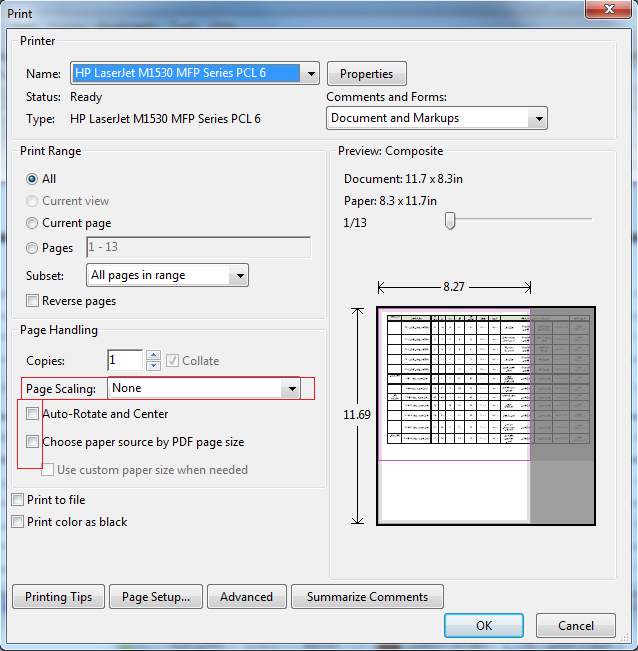
\includegraphics[width=0.7\textwidth]{Print-PDF}}}
 \caption{تنظیمات پرینتر در زمان چاپ.}\label{print}
 \end{figure}
\section{اگر سوالی داشتم، از کی بپرسم؟}
برای پرسیدن سوال‌های خود در مورد حروف‌چینی با زی‌پرشین،  می‌توانید به
 \href{http://qa.parsilatex.com}{سایت پرسش و پاسخ پارسی‌لاتک}%
\LTRfootnote{\url{http://qa.parsilatex.com}}
مراجعه کنید. شما هم می‌توانید روزی به سوال‌های دیگران در این سایت جواب بدهید.
    
در ادامه، برای فهم بیشتر مطالب، چند تعریف، قضیه و مثال آورده شده است. 
\begin{definition}
مجموعه همه ارزیابی‌های  (پیوسته)  روی $(X,\tau)$، دامنه توانی احتمالی
\index{دامنه توانی احتمالی}
$ X $
نامیده می‌شود.
\end{definition}
\begin{theorem}[باناخ-آلااغلو]
\index{قضیه باناخ-آلااغلو}
اگر $ V $ یک همسایگی $ 0 $ در فضای برداری 
\index{فضای!برداری}
 توپولوژیکی $ X $ باشد و 
\begin{equation}\label{eq1}
K=\left\lbrace \Lambda \in X^{*}:|\Lambda x|\leqslant 1 ; \ \forall x\in V\right\rbrace,
\end{equation}
آنگاه $ K $،  ضعیف*-فشرده است که در آن، $ X^{*} $ دوگان
\index{فضای!دوگان}
 فضای برداری توپولوژیکی $ X $ است به ‌طوری که عناصر آن،  تابعی‌های 
خطی پیوسته
\index{تابعی خطی پیوسته}
 روی $X$ هستند.
\end{theorem}
تساوی \eqref{eq1} یکی از مهم‌ترین تساوی‌ها در آنالیز تابعی است که در ادامه، به وفور از آن استفاده می‌شود.
\begin{example}
برای هر فضای مرتب، گردایه 
$$U:=\left\lbrace U\in O: U=\uparrow U\right\rbrace $$
از مجموعه‌های بالایی باز، یک توپولوژی تعریف می‌کند که از توپولوژی اصلی، درشت‌تر  است.
\end{example}
حال تساوی 
\begin{equation}\label{eq2}
\sum_{n=1}^{+\infty} 3^{n}x+70x=\int_{1}^{n}8nx+\exp{(2nx)}
\end{equation}
را در نظر بگیرید. با مقایسه تساوی \eqref{eq2} با تساوی \eqref{eq1} می‌توان نتیجه گرفت که ...
!
 قرار دهید.
\section{از کجا شروع کنم؟}
قبل از هر چیز، بدیهی است که باید یک توزیع تِک مناسب مانند 
\verb!Live TeX!
و یک ویرایش‌گر تِک مانند
\verb!Texmaker!
را روی سیستم خود نصب کنید.  نسخه بهینه شده \verb!Texmaker!  را می‌توانید  از سایت 
 \href{http://www.parsilatex.com}{پارسی‌لاتک}%
\LTRfootnote{\url{http://www.parsilatex.com}}
 و \verb!Live TeX!  را هم می‌توانید از 
 \href{http://www.tug.org/texlive}{سایت رسمی آن}%
\LTRfootnote{\url{http://www.tug.org/texlive}}
 دانلود کنید.
 
در مرحله بعد، سعی کنید که  یک پشتیبان از پوشه 
\LRE{\verb!yazd-thesis!}
 بگیرید و آن را در یک جایی از هارددیسک سیستم خود ذخیره کنید تا در صورت خراب کردن فایل‌هایی که در حال حاضر، با آن‌ها کار می‌کنید، همه چیز را از 
 دست ندهید.
 
 حال اگر نوشتن پایان‌نامه یا رساله اولین تجربه شما از کار با لاتک است، توصیه می‌شود که یک‌بار به طور سرسری، کتاب «%
\href{http://mirror.ctan.org/tex-archive/info/lshort/persian/lshort.pdf}{مقدمه‌ای نه چندان کوتاه بر
\lr{\LaTeXe}}\LTRfootnote{\url{http://mirror.ctan.org/tex-archive/info/lshort/persian/lshort.pdf}}»
   ترجمه دکتر مهدی امیدعلی، عضو هیات علمی دانشگاه شاهد را مطالعه کنید. این کتاب، کتاب بسیار کاملی است که خیلی از نیازهای شما در ارتباط با حروف‌چینی را برطرف می‌کند.
 
 
بعد از موارد گفته شده، فایل 
\LRE{\verb!yazd-thesis.tex!}
و
\LRE{\verb!fainfo!}
را باز کنید و مشخصات پایان‌نامه خود مثل نام، نام خانوادگی، عنوان پایان‌نامه و ... را جایگزین مشخصات موجود در فایل
\LRE{\verb!fainfo!}
 کنید. دقت داشته باشید که نیازی نیست 
نگران چینش این مشخصات در فایل پی‌دی‌اف خروجی باشید. فایل 
\LRE{\verb!yazd-thesis.cls!}
همه این کارها را به طور خودکار برای شما انجام می‌دهد. در ضمن، موقع تغییر دادن دستورهای داخل فایل
\LRE{\verb!fainfo!}
 کاملاً  دقت کنید. این دستورها، خیلی حساس هستند و ممکن است با یک تغییر کوچک، موقع اجرا، خطا بگیرید. برای دیدن خروجی کار، فایل 
\LRE{\verb!fainfo!}
 را 
\verb!Save!، 
(نه 
\verb!As Save!)
کنید و بعد به فایل 
\LRE{\verb!yazd-thesis.tex!}
برگشته و آن را اجرا کنید. حال اگر می‌خواهید مشخصات انگلیسی پایان‌نامه یا رساله را هم عوض کنید، فایل 
\LRE{\verb!eninfo!}
را باز کنید و مشخصات داخل آن را تغییر دهید.
در اینجا هم برای دیدن خروجی، باید این فایل را 
\verb!Save!
کرده و بعد به فایل 
\LRE{\verb!yazd-thesis.tex!}
برگشته و آن را اجرا کرد.

برای راحتی بیشتر، 
فایل 
\LRE{\verb!yazd-thesis.cls!}
طوری طراحی شده است که کافی است فقط  یک‌بار مشخصات پایان‌نامه یا رساله  را وارد کنید. هر جای دیگر که لازم به درج این مشخصات باشد، این مشخصات به طور خودکار درج می‌شود. با این حال، اگر مایل بودید، می‌توانید تنظیمات موجود را تغییر دهید. توجه داشته باشید که اگر کاربر مبتدی هستید و یا با ساختار فایل‌های  
\verb!cls!
 آشنایی ندارید، به هیچ وجه به این فایل، یعنی فایل 
\LRE{\verb!yazd-thesis.cls!}
دست نزنید.

نکته دیگری که باید به آن توجه کنید این است که چنانچه قصد حروف‌چینی رساله دکتری را دارید، 
 در فایل 
\LRE{\verb!yazd-thesis.tex!}
باید گزینه
\verb!msc!
را پاک کنید. با این کار، تنظیمات مربوطه به طور خودکار  اعمال می‌شود.    
\section{مطالب پایان‌نامه یا رساله را چطور بنویسم؟}
\subsection{نوشتن فصل‌ها}
همان‌طور که در بخش \ref{sec2} گفته شد، برای جلوگیری از شلوغی و سردرگمی کاربر در هنگام حروف‌چینی، قسمت‌های مختلف پایان‌نامه یا رساله از جمله فصل‌ها، در فایل‌های جداگانه‌ای قرار داده شده‌اند. 
بنابراین، اگر می‌خواهید مثلاً مطالب فصل ۱ را تایپ کنید، باید فایل‌های 
\LRE{\verb!yazd-thesis.tex!}
و
\verb!chapter1!
را باز کنید و محتویات داخل فایل 
\verb!chapter1!
را پاک کرده و مطالب خود را تایپ کنید. توجه کنید که همان‌طور که قبلاً هم گفته شد، تنها فایل قابل اجرا، فایل 
\LRE{\verb!yazd-thesis.tex!}
است. لذا برای دیدن حاصل (خروجی) فایل خود، باید فایل  
\verb!chapter1!
را 
\verb!Save!
کرده و سپس فایل 
\LRE{\verb!yazd-thesis.tex!}
را اجرا کنید. یک نکته بدیهی که در اینجا وجود دارد، این است که لازم نیست که فصل‌های پایان‌نامه یا رساله را به ترتیب تایپ کنید. می‌توانید ابتدا مطالب فصل ۳ را تایپ کنید و سپس مطالب فصل ۱ را تایپ کنید. 

نکته بسیار مهمی که در اینجا باید گفته شود این است که سیستم \lr{\TeX}، محتویات یک فایل تِک را به ترتیب پردازش می‌کند. به عنوان مثال، اگه فایلی، دارای ۴ خط دستور باشد، ابتدا خط ۱، بعد خط ۲، بعد خط ۳ و در آخر، خط ۴ پردازش می‌شود. بنابراین، اگر مثلاً مشغول تایپ مطالب فصل ۳ هستید، بهتر است
که دو دستور 
\verb!% Sample University of Calgary Thesis
% This file contains CHAPTER ONE

\chapter{Introduction}

\epigraph{Lorem ipsum dolor sit amet,
consectetuer adipiscing elit.}{Anonymous}

The text above is an \emph{epigraph}. In this typeface, you can have
text in \textbf{boldface}, \emph{italics}, \textbf{\emph{bold
    italics}}, \textsl{slanted}, and \textsc{Small Caps}.

\section{Literature Review}

\blindtext\pagenote{\blindtext}

\blindtext[2]

\begin{defn}
A group~$G$ is said to be \emph{abelian} (or \emph{commutative}) if
for every $a, b \in G$, $a \cdot b = b \cdot a$.
\end{defn}

\blindtext[2]

\section{Contributions of the Thesis}

\blindtext[3]

\begin{table}
  \begin{center}
  \begin{tabular}{c|c}
    A & B \\
    \hline
    1 & 2
  \end{tabular}
  \end{center}
  \caption{Letters and numbers}
\end{table}

\blindtext[3]
!
و
\verb!\chapter{فضاهای فشرده پایدار و فضاهای مرتب فشرده}
\thispagestyle{empty}
\section{فضاهای فشرده پایدار}
یک فضای توپولوژیک جزئاً مرتب (یا به طور خلاصه، فضای مرتب)، از دیدگاه آبرامسکی
\cite{abramsky2}،
مجموعه‌ای مانند $ X $ همراه 
با یک توپولوژی $ \mathcal{O} $ و یک ترتیب $ \leq $ است به طوری که گراف ترتیب در $X\times X  $ بسته باشد. بنابراین ...
\section{فضاهای مرتب فشرده}
در این  بخش به بیان ...!
را در فایل 
\LRE{\verb!yazd-thesis.tex!}،
غیرفعال%
\RTLfootnote{
برای غیرفعال کردن یک دستور، کافی است پشت آن، یک علامت
\%
 بگذارید.
}
 کنید. زیرا در غیر این صورت، ابتدا مطالب فصل ۱ و ۲ پردازش شده (که به درد ما نمی‌خورد؛ چون ما می‌خواهیم خروجی فصل ۳ را ببینیم) و سپس مطالب فصل ۳ پردازش می‌شود و این کار باعث طولانی شدن زمان اجرا می‌شود. زیرا هر چقدر حجم فایل اجرا شده، بیشتر باشد، زمان بیشتری هم برای اجرای آن، صرف می‌شود.
\subsection{مراجع}
مرجع \cite{Omidali82phdThesis} یک نمونه پروژه دکترا و مرجع \cite{Vahedi87} یک نمونه مقاله مجله فارسی است.
مرجع \cite{Amintoosi87afzayesh}  یک نمونه  مقاله کنفرانس فارسی و
مرجع \cite{vahid90} یک نمونه کتاب فارسی است. مرجع \cite{Khalighi07MscThesis} یک نمونه پروژه کارشناسی ارشد انگلیسی و
\cite{Khalighi87xepersian} هم یک نمونه متفرقه  می‌باشند.

مرجع \cite{Gonzalez02book} یک نمونه کتاب لاتین است که از آنجا که دارای فیلد \lr{authorfa} است، نام نویسندگان آن در استیلهای \lr{asa-fa}، \lr{plainnat-fa} و \lr{chicago-fa} به فارسی دیده می‌شود. مرجع \cite{Baker02limits} مقاله انگلیسی است که معادل فارسی نام نویسندگان آن ذکر نشده بوده است.

برای تولید مراجع باید از دستور \lr{bibtex} استفاده کنید. در صورتی که بخواهید مراجع فارسی قبل از
مراجع انگلیسی بیایند، باید به جای دستور \lr{bibtex thesis} از دستور زیر استفاده کنید:
\begin{latin}
\lr{bibtex8 -W -c cp1256fa thesis}
\end{latin}
\subsection{واژه‌نامه فارسی به انگلیسی و برعکس}
برای وارد کردن واژه‌نامه فارسی به انگلیسی و برعکس، چنانچه کاربر مبتدی هستید، بهتر است مانند روش بکار رفته در فایل‌های 
\verb!dicfa2en!
و
\verb!dicen2fa!
عمل کنید. اما چنانچه کاربر پیشرفته هستید، بهتر است از بسته
\verb!glossaries!
استفاده کنید. راهنمای این بسته را می‌توانید به راحتی و با یک جستجوی ساده در اینترنت پیدا کنید.
\subsection{نمایه}
برای وارد کردن نمایه، باید از 
\verb!xindy!
استفاده کنید. زیرا 
\verb!MakeIndex!
با حروف «گ»، «چ»، «پ»، «ژ» و «ک» مشکل دارد و ترتیب الفبایی این حروف را رعایت نمی‌کند. همچنین، فاصله بین هر گروه از کلمات در 
\verb!MakeIndex!،
به درستی رعایت نمی‌شود که باعث زشت شدن حروف‌چینی این قسمت می‌شود. راهنمای چگونگی کار با 
\verb!xindy! 
را می‌توانید در تالار گفتگوی پارسی‌لاتک، پیدا کنید.

دستور مربوطه به صورت زیر است:

\begin{latin}
\footnotesize
\begin{verbatim}
xindy -L persian-variant2 -C utf8 -M texindy -M page-ranges yazd-thesis.idx
\end{verbatim}
\end{latin}

\subsection{تعریف نمادها و ایجاد فهرست نمادها}
ابتدا باید نمادها یکی یکی با استفاده از دستور
\LRE{\verb!\psymbol{<symbol>}{<description>}!}
در متن کتاب تعریف شوند. در این دستور منظور از 
\LRE{\verb!<symbol>!}
خود نماد است که در صورت ریاضی بودن آن، از 
\verb!$...$!
و در صورت ریاضی نبودن آن از دستور
\verb!\lr{...}!
برای نوشتن آن استفاده می‌شود. 
\LRE{\verb!<description>!}
هم توضیح و یا معنی نماد است. این دستور، نماد را در متن کتاب  چاپ می‌کند. دستور
\verb!\listofsymbols%[3em]!
در فایل
\textsf{yazd-thesis.tex}
هم فهرست نمادها را چاپ می‌کند. 
مقدار
\verb![3em]!
را می‌توانید در پایان کار، بسته به پهنای نمادها 
کم و زیاد کنید. 


\section{چاپ فایل پی دی اف}
فایل پی دی اف حاصل از این بسته، مطمئناً مطابق با آیین‌نامه نگارش پایان‌نامه دانشگاه یزد
است و این امر توسط کارشناسان مرکز تحصیلات تکمیلی دانشگاه یزد تایید شده است.
اما چاپ فایل پی دی اف حاصل نیز باید به صورتی باشد که در خروجی تغییراتی داده نشود و نسخۀ
چاپ شده نیز مطابق با دستورالعمل باشد. 

 مشکل اصلی این است که برخی تنظیمات پرینتر، باعث ایجاد تغییرات در محصول نهایی می‌شود.
  حتی تغییر پرینتر نیز گاهی آنها را عوض می‌کند. 
 نکته‌ای که مشکل را حل می‌کند این است که، اولا حتما مطئن شوید 
 که اندازه کاغذ انتخابی در موقع پرینت، همان A4 باشد و ثانیا تمام گزینه‌های مربوط 
 به Page Handling  را غیرفعال کنید. نمونه به صورت شکل~\ref{print} است.
دقت کنید که بسته به پرینتر شما ممکن است موارد دیگری نظیر shrinking  و غیره نیز 
موجود باشد که باید همه غیر فعال شوند.
با این ترتیب، مطمئنا حاشیه‌ها مطابق حاشیه‌ها در فایل پی دی اف خواهد بود.
\begin{figure}[!h]
 {\centerline{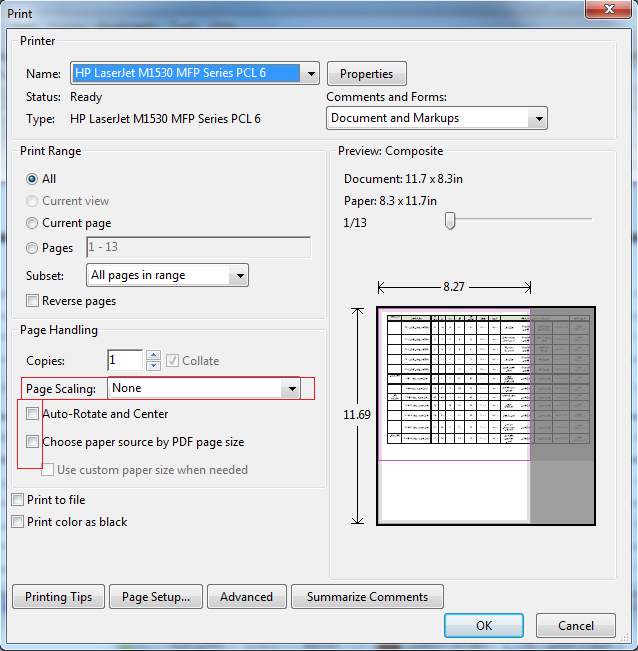
\includegraphics[width=0.7\textwidth]{Print-PDF}}}
 \caption{تنظیمات پرینتر در زمان چاپ.}\label{print}
 \end{figure}
\section{اگر سوالی داشتم، از کی بپرسم؟}
برای پرسیدن سوال‌های خود در مورد حروف‌چینی با زی‌پرشین،  می‌توانید به
 \href{http://qa.parsilatex.com}{سایت پرسش و پاسخ پارسی‌لاتک}%
\LTRfootnote{\url{http://qa.parsilatex.com}}
مراجعه کنید. شما هم می‌توانید روزی به سوال‌های دیگران در این سایت جواب بدهید.
    
در ادامه، برای فهم بیشتر مطالب، چند تعریف، قضیه و مثال آورده شده است. 
\begin{definition}
مجموعه همه ارزیابی‌های  (پیوسته)  روی $(X,\tau)$، دامنه توانی احتمالی
\index{دامنه توانی احتمالی}
$ X $
نامیده می‌شود.
\end{definition}
\begin{theorem}[باناخ-آلااغلو]
\index{قضیه باناخ-آلااغلو}
اگر $ V $ یک همسایگی $ 0 $ در فضای برداری 
\index{فضای!برداری}
 توپولوژیکی $ X $ باشد و 
\begin{equation}\label{eq1}
K=\left\lbrace \Lambda \in X^{*}:|\Lambda x|\leqslant 1 ; \ \forall x\in V\right\rbrace,
\end{equation}
آنگاه $ K $،  ضعیف*-فشرده است که در آن، $ X^{*} $ دوگان
\index{فضای!دوگان}
 فضای برداری توپولوژیکی $ X $ است به ‌طوری که عناصر آن،  تابعی‌های 
خطی پیوسته
\index{تابعی خطی پیوسته}
 روی $X$ هستند.
\end{theorem}
تساوی \eqref{eq1} یکی از مهم‌ترین تساوی‌ها در آنالیز تابعی است که در ادامه، به وفور از آن استفاده می‌شود.
\begin{example}
برای هر فضای مرتب، گردایه 
$$U:=\left\lbrace U\in O: U=\uparrow U\right\rbrace $$
از مجموعه‌های بالایی باز، یک توپولوژی تعریف می‌کند که از توپولوژی اصلی، درشت‌تر  است.
\end{example}
حال تساوی 
\begin{equation}\label{eq2}
\sum_{n=1}^{+\infty} 3^{n}x+70x=\int_{1}^{n}8nx+\exp{(2nx)}
\end{equation}
را در نظر بگیرید. با مقایسه تساوی \eqref{eq2} با تساوی \eqref{eq1} می‌توان نتیجه گرفت که ...
!
 قرار دهید.
\section{از کجا شروع کنم؟}
قبل از هر چیز، بدیهی است که باید یک توزیع تِک مناسب مانند 
\verb!Live TeX!
و یک ویرایش‌گر تِک مانند
\verb!Texmaker!
را روی سیستم خود نصب کنید.  نسخه بهینه شده \verb!Texmaker!  را می‌توانید  از سایت 
 \href{http://www.parsilatex.com}{پارسی‌لاتک}%
\LTRfootnote{\url{http://www.parsilatex.com}}
 و \verb!Live TeX!  را هم می‌توانید از 
 \href{http://www.tug.org/texlive}{سایت رسمی آن}%
\LTRfootnote{\url{http://www.tug.org/texlive}}
 دانلود کنید.
 
در مرحله بعد، سعی کنید که  یک پشتیبان از پوشه 
\LRE{\verb!yazd-thesis!}
 بگیرید و آن را در یک جایی از هارددیسک سیستم خود ذخیره کنید تا در صورت خراب کردن فایل‌هایی که در حال حاضر، با آن‌ها کار می‌کنید، همه چیز را از 
 دست ندهید.
 
 حال اگر نوشتن پایان‌نامه یا رساله اولین تجربه شما از کار با لاتک است، توصیه می‌شود که یک‌بار به طور سرسری، کتاب «%
\href{http://mirror.ctan.org/tex-archive/info/lshort/persian/lshort.pdf}{مقدمه‌ای نه چندان کوتاه بر
\lr{\LaTeXe}}\LTRfootnote{\url{http://mirror.ctan.org/tex-archive/info/lshort/persian/lshort.pdf}}»
   ترجمه دکتر مهدی امیدعلی، عضو هیات علمی دانشگاه شاهد را مطالعه کنید. این کتاب، کتاب بسیار کاملی است که خیلی از نیازهای شما در ارتباط با حروف‌چینی را برطرف می‌کند.
 
 
بعد از موارد گفته شده، فایل 
\LRE{\verb!yazd-thesis.tex!}
و
\LRE{\verb!fainfo!}
را باز کنید و مشخصات پایان‌نامه خود مثل نام، نام خانوادگی، عنوان پایان‌نامه و ... را جایگزین مشخصات موجود در فایل
\LRE{\verb!fainfo!}
 کنید. دقت داشته باشید که نیازی نیست 
نگران چینش این مشخصات در فایل پی‌دی‌اف خروجی باشید. فایل 
\LRE{\verb!yazd-thesis.cls!}
همه این کارها را به طور خودکار برای شما انجام می‌دهد. در ضمن، موقع تغییر دادن دستورهای داخل فایل
\LRE{\verb!fainfo!}
 کاملاً  دقت کنید. این دستورها، خیلی حساس هستند و ممکن است با یک تغییر کوچک، موقع اجرا، خطا بگیرید. برای دیدن خروجی کار، فایل 
\LRE{\verb!fainfo!}
 را 
\verb!Save!، 
(نه 
\verb!As Save!)
کنید و بعد به فایل 
\LRE{\verb!yazd-thesis.tex!}
برگشته و آن را اجرا کنید. حال اگر می‌خواهید مشخصات انگلیسی پایان‌نامه یا رساله را هم عوض کنید، فایل 
\LRE{\verb!eninfo!}
را باز کنید و مشخصات داخل آن را تغییر دهید.
در اینجا هم برای دیدن خروجی، باید این فایل را 
\verb!Save!
کرده و بعد به فایل 
\LRE{\verb!yazd-thesis.tex!}
برگشته و آن را اجرا کرد.

برای راحتی بیشتر، 
فایل 
\LRE{\verb!yazd-thesis.cls!}
طوری طراحی شده است که کافی است فقط  یک‌بار مشخصات پایان‌نامه یا رساله  را وارد کنید. هر جای دیگر که لازم به درج این مشخصات باشد، این مشخصات به طور خودکار درج می‌شود. با این حال، اگر مایل بودید، می‌توانید تنظیمات موجود را تغییر دهید. توجه داشته باشید که اگر کاربر مبتدی هستید و یا با ساختار فایل‌های  
\verb!cls!
 آشنایی ندارید، به هیچ وجه به این فایل، یعنی فایل 
\LRE{\verb!yazd-thesis.cls!}
دست نزنید.

نکته دیگری که باید به آن توجه کنید این است که چنانچه قصد حروف‌چینی رساله دکتری را دارید، 
 در فایل 
\LRE{\verb!yazd-thesis.tex!}
باید گزینه
\verb!msc!
را پاک کنید. با این کار، تنظیمات مربوطه به طور خودکار  اعمال می‌شود.    
\section{مطالب پایان‌نامه یا رساله را چطور بنویسم؟}
\subsection{نوشتن فصل‌ها}
همان‌طور که در بخش \ref{sec2} گفته شد، برای جلوگیری از شلوغی و سردرگمی کاربر در هنگام حروف‌چینی، قسمت‌های مختلف پایان‌نامه یا رساله از جمله فصل‌ها، در فایل‌های جداگانه‌ای قرار داده شده‌اند. 
بنابراین، اگر می‌خواهید مثلاً مطالب فصل ۱ را تایپ کنید، باید فایل‌های 
\LRE{\verb!yazd-thesis.tex!}
و
\verb!chapter1!
را باز کنید و محتویات داخل فایل 
\verb!chapter1!
را پاک کرده و مطالب خود را تایپ کنید. توجه کنید که همان‌طور که قبلاً هم گفته شد، تنها فایل قابل اجرا، فایل 
\LRE{\verb!yazd-thesis.tex!}
است. لذا برای دیدن حاصل (خروجی) فایل خود، باید فایل  
\verb!chapter1!
را 
\verb!Save!
کرده و سپس فایل 
\LRE{\verb!yazd-thesis.tex!}
را اجرا کنید. یک نکته بدیهی که در اینجا وجود دارد، این است که لازم نیست که فصل‌های پایان‌نامه یا رساله را به ترتیب تایپ کنید. می‌توانید ابتدا مطالب فصل ۳ را تایپ کنید و سپس مطالب فصل ۱ را تایپ کنید. 

نکته بسیار مهمی که در اینجا باید گفته شود این است که سیستم \lr{\TeX}، محتویات یک فایل تِک را به ترتیب پردازش می‌کند. به عنوان مثال، اگه فایلی، دارای ۴ خط دستور باشد، ابتدا خط ۱، بعد خط ۲، بعد خط ۳ و در آخر، خط ۴ پردازش می‌شود. بنابراین، اگر مثلاً مشغول تایپ مطالب فصل ۳ هستید، بهتر است
که دو دستور 
\verb!% Sample University of Calgary Thesis
% This file contains CHAPTER ONE

\chapter{Introduction}

\epigraph{Lorem ipsum dolor sit amet,
consectetuer adipiscing elit.}{Anonymous}

The text above is an \emph{epigraph}. In this typeface, you can have
text in \textbf{boldface}, \emph{italics}, \textbf{\emph{bold
    italics}}, \textsl{slanted}, and \textsc{Small Caps}.

\section{Literature Review}

\blindtext\pagenote{\blindtext}

\blindtext[2]

\begin{defn}
A group~$G$ is said to be \emph{abelian} (or \emph{commutative}) if
for every $a, b \in G$, $a \cdot b = b \cdot a$.
\end{defn}

\blindtext[2]

\section{Contributions of the Thesis}

\blindtext[3]

\begin{table}
  \begin{center}
  \begin{tabular}{c|c}
    A & B \\
    \hline
    1 & 2
  \end{tabular}
  \end{center}
  \caption{Letters and numbers}
\end{table}

\blindtext[3]
!
و
\verb!\chapter{فضاهای فشرده پایدار و فضاهای مرتب فشرده}
\thispagestyle{empty}
\section{فضاهای فشرده پایدار}
یک فضای توپولوژیک جزئاً مرتب (یا به طور خلاصه، فضای مرتب)، از دیدگاه آبرامسکی
\cite{abramsky2}،
مجموعه‌ای مانند $ X $ همراه 
با یک توپولوژی $ \mathcal{O} $ و یک ترتیب $ \leq $ است به طوری که گراف ترتیب در $X\times X  $ بسته باشد. بنابراین ...
\section{فضاهای مرتب فشرده}
در این  بخش به بیان ...!
را در فایل 
\LRE{\verb!yazd-thesis.tex!}،
غیرفعال%
\RTLfootnote{
برای غیرفعال کردن یک دستور، کافی است پشت آن، یک علامت
\%
 بگذارید.
}
 کنید. زیرا در غیر این صورت، ابتدا مطالب فصل ۱ و ۲ پردازش شده (که به درد ما نمی‌خورد؛ چون ما می‌خواهیم خروجی فصل ۳ را ببینیم) و سپس مطالب فصل ۳ پردازش می‌شود و این کار باعث طولانی شدن زمان اجرا می‌شود. زیرا هر چقدر حجم فایل اجرا شده، بیشتر باشد، زمان بیشتری هم برای اجرای آن، صرف می‌شود.
\subsection{مراجع}
مرجع \cite{Omidali82phdThesis} یک نمونه پروژه دکترا و مرجع \cite{Vahedi87} یک نمونه مقاله مجله فارسی است.
مرجع \cite{Amintoosi87afzayesh}  یک نمونه  مقاله کنفرانس فارسی و
مرجع \cite{vahid90} یک نمونه کتاب فارسی است. مرجع \cite{Khalighi07MscThesis} یک نمونه پروژه کارشناسی ارشد انگلیسی و
\cite{Khalighi87xepersian} هم یک نمونه متفرقه  می‌باشند.

مرجع \cite{Gonzalez02book} یک نمونه کتاب لاتین است که از آنجا که دارای فیلد \lr{authorfa} است، نام نویسندگان آن در استیلهای \lr{asa-fa}، \lr{plainnat-fa} و \lr{chicago-fa} به فارسی دیده می‌شود. مرجع \cite{Baker02limits} مقاله انگلیسی است که معادل فارسی نام نویسندگان آن ذکر نشده بوده است.

برای تولید مراجع باید از دستور \lr{bibtex} استفاده کنید. در صورتی که بخواهید مراجع فارسی قبل از
مراجع انگلیسی بیایند، باید به جای دستور \lr{bibtex thesis} از دستور زیر استفاده کنید:
\begin{latin}
\lr{bibtex8 -W -c cp1256fa thesis}
\end{latin}
\subsection{واژه‌نامه فارسی به انگلیسی و برعکس}
برای وارد کردن واژه‌نامه فارسی به انگلیسی و برعکس، چنانچه کاربر مبتدی هستید، بهتر است مانند روش بکار رفته در فایل‌های 
\verb!dicfa2en!
و
\verb!dicen2fa!
عمل کنید. اما چنانچه کاربر پیشرفته هستید، بهتر است از بسته
\verb!glossaries!
استفاده کنید. راهنمای این بسته را می‌توانید به راحتی و با یک جستجوی ساده در اینترنت پیدا کنید.
\subsection{نمایه}
برای وارد کردن نمایه، باید از 
\verb!xindy!
استفاده کنید. زیرا 
\verb!MakeIndex!
با حروف «گ»، «چ»، «پ»، «ژ» و «ک» مشکل دارد و ترتیب الفبایی این حروف را رعایت نمی‌کند. همچنین، فاصله بین هر گروه از کلمات در 
\verb!MakeIndex!،
به درستی رعایت نمی‌شود که باعث زشت شدن حروف‌چینی این قسمت می‌شود. راهنمای چگونگی کار با 
\verb!xindy! 
را می‌توانید در تالار گفتگوی پارسی‌لاتک، پیدا کنید.

دستور مربوطه به صورت زیر است:

\begin{latin}
\footnotesize
\begin{verbatim}
xindy -L persian-variant2 -C utf8 -M texindy -M page-ranges yazd-thesis.idx
\end{verbatim}
\end{latin}

\subsection{تعریف نمادها و ایجاد فهرست نمادها}
ابتدا باید نمادها یکی یکی با استفاده از دستور
\LRE{\verb!\psymbol{<symbol>}{<description>}!}
در متن کتاب تعریف شوند. در این دستور منظور از 
\LRE{\verb!<symbol>!}
خود نماد است که در صورت ریاضی بودن آن، از 
\verb!$...$!
و در صورت ریاضی نبودن آن از دستور
\verb!\lr{...}!
برای نوشتن آن استفاده می‌شود. 
\LRE{\verb!<description>!}
هم توضیح و یا معنی نماد است. این دستور، نماد را در متن کتاب  چاپ می‌کند. دستور
\verb!\listofsymbols%[3em]!
در فایل
\textsf{yazd-thesis.tex}
هم فهرست نمادها را چاپ می‌کند. 
مقدار
\verb![3em]!
را می‌توانید در پایان کار، بسته به پهنای نمادها 
کم و زیاد کنید. 


\section{چاپ فایل پی دی اف}
فایل پی دی اف حاصل از این بسته، مطمئناً مطابق با آیین‌نامه نگارش پایان‌نامه دانشگاه یزد
است و این امر توسط کارشناسان مرکز تحصیلات تکمیلی دانشگاه یزد تایید شده است.
اما چاپ فایل پی دی اف حاصل نیز باید به صورتی باشد که در خروجی تغییراتی داده نشود و نسخۀ
چاپ شده نیز مطابق با دستورالعمل باشد. 

 مشکل اصلی این است که برخی تنظیمات پرینتر، باعث ایجاد تغییرات در محصول نهایی می‌شود.
  حتی تغییر پرینتر نیز گاهی آنها را عوض می‌کند. 
 نکته‌ای که مشکل را حل می‌کند این است که، اولا حتما مطئن شوید 
 که اندازه کاغذ انتخابی در موقع پرینت، همان A4 باشد و ثانیا تمام گزینه‌های مربوط 
 به Page Handling  را غیرفعال کنید. نمونه به صورت شکل~\ref{print} است.
دقت کنید که بسته به پرینتر شما ممکن است موارد دیگری نظیر shrinking  و غیره نیز 
موجود باشد که باید همه غیر فعال شوند.
با این ترتیب، مطمئنا حاشیه‌ها مطابق حاشیه‌ها در فایل پی دی اف خواهد بود.
\begin{figure}[!h]
 {\centerline{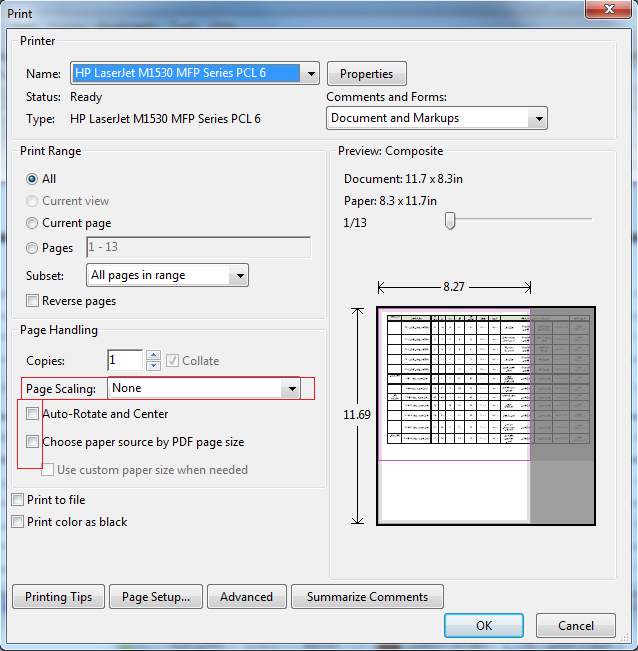
\includegraphics[width=0.7\textwidth]{Print-PDF}}}
 \caption{تنظیمات پرینتر در زمان چاپ.}\label{print}
 \end{figure}
\section{اگر سوالی داشتم، از کی بپرسم؟}
برای پرسیدن سوال‌های خود در مورد حروف‌چینی با زی‌پرشین،  می‌توانید به
 \href{http://qa.parsilatex.com}{سایت پرسش و پاسخ پارسی‌لاتک}%
\LTRfootnote{\url{http://qa.parsilatex.com}}
مراجعه کنید. شما هم می‌توانید روزی به سوال‌های دیگران در این سایت جواب بدهید.
    
در ادامه، برای فهم بیشتر مطالب، چند تعریف، قضیه و مثال آورده شده است. 
\begin{definition}
مجموعه همه ارزیابی‌های  (پیوسته)  روی $(X,\tau)$، دامنه توانی احتمالی
\index{دامنه توانی احتمالی}
$ X $
نامیده می‌شود.
\end{definition}
\begin{theorem}[باناخ-آلااغلو]
\index{قضیه باناخ-آلااغلو}
اگر $ V $ یک همسایگی $ 0 $ در فضای برداری 
\index{فضای!برداری}
 توپولوژیکی $ X $ باشد و 
\begin{equation}\label{eq1}
K=\left\lbrace \Lambda \in X^{*}:|\Lambda x|\leqslant 1 ; \ \forall x\in V\right\rbrace,
\end{equation}
آنگاه $ K $،  ضعیف*-فشرده است که در آن، $ X^{*} $ دوگان
\index{فضای!دوگان}
 فضای برداری توپولوژیکی $ X $ است به ‌طوری که عناصر آن،  تابعی‌های 
خطی پیوسته
\index{تابعی خطی پیوسته}
 روی $X$ هستند.
\end{theorem}
تساوی \eqref{eq1} یکی از مهم‌ترین تساوی‌ها در آنالیز تابعی است که در ادامه، به وفور از آن استفاده می‌شود.
\begin{example}
برای هر فضای مرتب، گردایه 
$$U:=\left\lbrace U\in O: U=\uparrow U\right\rbrace $$
از مجموعه‌های بالایی باز، یک توپولوژی تعریف می‌کند که از توپولوژی اصلی، درشت‌تر  است.
\end{example}
حال تساوی 
\begin{equation}\label{eq2}
\sum_{n=1}^{+\infty} 3^{n}x+70x=\int_{1}^{n}8nx+\exp{(2nx)}
\end{equation}
را در نظر بگیرید. با مقایسه تساوی \eqref{eq2} با تساوی \eqref{eq1} می‌توان نتیجه گرفت که ...
!
 قرار دهید.
\section{از کجا شروع کنم؟}
قبل از هر چیز، بدیهی است که باید یک توزیع تِک مناسب مانند 
\verb!Live TeX!
و یک ویرایش‌گر تِک مانند
\verb!Texmaker!
را روی سیستم خود نصب کنید.  نسخه بهینه شده \verb!Texmaker!  را می‌توانید  از سایت 
 \href{http://www.parsilatex.com}{پارسی‌لاتک}%
\LTRfootnote{\url{http://www.parsilatex.com}}
 و \verb!Live TeX!  را هم می‌توانید از 
 \href{http://www.tug.org/texlive}{سایت رسمی آن}%
\LTRfootnote{\url{http://www.tug.org/texlive}}
 دانلود کنید.
 
در مرحله بعد، سعی کنید که  یک پشتیبان از پوشه 
\LRE{\verb!tabriz-thesis!}
 بگیرید و آن را در یک جایی از هارددیسک سیستم خود ذخیره کنید تا در صورت خراب کردن فایل‌هایی که در حال حاضر، با آن‌ها کار می‌کنید، همه چیز را از 
 دست ندهید.
 
 حال اگر نوشتن \پ اولین تجربه شما از کار با لاتک است، توصیه می‌شود که یک‌بار به طور سرسری، کتاب «%
\href{http://www.tug.ctan.org/tex-archive/info/lshort/persian/lshort.pdf}{مقدمه‌ای نه چندان کوتاه بر
\lr{\LaTeXe}}\LTRfootnote{\url{http://www.tug.ctan.org/tex-archive/info/lshort/persian/lshort.pdf}}»
   ترجمه دکتر مهدی امیدعلی، عضو هیات علمی دانشگاه شاهد را مطالعه کنید. این کتاب، کتاب بسیار کاملی است که خیلی از نیازهای شما در ارتباط با حروف‌چینی را برطرف می‌کند.
 
 
بعد از موارد گفته شده، فایل 
\LRE{\verb!tabriz-thesis.tex!}
و
\LRE{\verb!fa-title!}
را باز کنید و مشخصات پایان‌نامه خود مثل نام، نام خانوادگی، عنوان پایان‌نامه و ... را جایگزین مشخصات موجود در فایل
\LRE{\verb!fa-title!}
 کنید. دقت داشته باشید که نیازی نیست 
نگران چینش این مشخصات در فایل پی‌دی‌اف خروجی باشید. فایل 
\LRE{\verb!tabriz-thesis.cls!}
همه این کارها را به طور خودکار برای شما انجام می‌دهد. در ضمن، موقع تغییر دادن دستورهای داخل فایل
\LRE{\verb!fa-title!}
 کاملاً دقت کنید. این دستورها، خیلی حساس هستند و ممکن است با یک تغییر کوچک، موقع اجرا، خطا بگیرید. برای دیدن خروجی کار، فایل 
\LRE{\verb!fa-title!}
 را 
\verb!Save!، 
(نه 
\verb!As Save!)
کنید و بعد به فایل 
\LRE{\verb!tabriz-thesis.tex!}
برگشته و آن را اجرا کنید. حال اگر می‌خواهید مشخصات انگلیسی \پ را هم عوض کنید، فایل 
\LRE{\verb!en-title!}
را باز کنید و مشخصات داخل آن را تغییر دهید.%
\RTLfootnote{
برای نوشتن پروژه کارشناسی، نیازی به وارد کردن مشخصات انگلیسی پروژه نیست. بنابراین، این مشخصات، به طور خودکار،
نادیده گرفته می‌شود.
}
 در اینجا هم برای دیدن خروجی، باید این فایل را 
\verb!Save!
کرده و بعد به فایل 
\LRE{\verb!tabriz-thesis.tex!}
برگشته و آن را اجرا کرد.

برای راحتی بیشتر، 
فایل 
\LRE{\verb!tabriz-thesis.cls!}
طوری طراحی شده است که کافی است فقط  یک‌بار مشخصات \پ  را وارد کنید. هر جای دیگر که لازم به درج این مشخصات باشد، این مشخصات به طور خودکار درج می‌شود. با این حال، اگر مایل بودید، می‌توانید تنظیمات موجود را تغییر دهید. توجه داشته باشید که اگر کاربر مبتدی هستید و یا با ساختار فایل‌های  
\verb!cls!
 آشنایی ندارید، به هیچ وجه به این فایل، یعنی فایل 
\LRE{\verb!tabriz-thesis.cls!}
دست نزنید.

نکته دیگری که باید به آن توجه کنید این است که در فایل 
\LRE{\verb!tabriz-thesis.cls!}،
سه گزینه به نام‌های
\verb!bsc!،
\verb!msc!
و
\verb!phd!
برای تایپ پروژه، پایان‌نامه و رساله،
طراحی شده است. بنابراین اگر قصد تایپ پروژه کارشناسی، پایان‌نامه یا رساله را دارید، 
 در فایل 
\LRE{\verb!tabriz-thesis.tex!}
باید به ترتیب از گزینه‌های
\verb!bsc!،
\verb!msc!
و
\verb!phd!
استفاده کنید. با انتخاب هر کدام از این گزینه‌ها، تنظیمات مربوط به آنها به طور خودکار، اعمل می‌شود.    
\section{مطالب \پ را چطور بنویسم؟}
\subsection{نوشتن فصل‌ها}
همان‌طور که در بخش \ref{sec2} گفته شد، برای جلوگیری از شلوغی و سردرگمی کاربر در هنگام حروف‌چینی، قسمت‌های مختلف \پ از جمله فصل‌ها، در فایل‌های جداگانه‌ای قرار داده شده‌اند. 
بنابراین، اگر می‌خواهید مثلاً مطالب فصل ۱ را تایپ کنید، باید فایل‌های 
\LRE{\verb!tabriz-thesis.tex!}
و
\verb!chapter1!
را باز کنید و محتویات داخل فایل 
\verb!chapter1!
را پاک کرده و مطالب خود را تایپ کنید. توجه کنید که همان‌طور که قبلاً هم گفته شد، تنها فایل قابل اجرا، فایل 
\LRE{\verb!tabriz-thesis.tex!}
است. لذا برای دیدن حاصل (خروجی) فایل خود، باید فایل  
\verb!chapter1!
را 
\verb!Save!
کرده و سپس فایل 
\LRE{\verb!tabriz-thesis.tex!}
را اجرا کنید. یک نکته بدیهی که در اینجا وجود دارد، این است که لازم نیست که فصل‌های \پ را به ترتیب تایپ کنید. می‌توانید ابتدا مطالب فصل ۳ را تایپ کنید و سپس مطالب فصل ۱ را تایپ کنید. 

نکته بسیار مهمی که در اینجا باید گفته شود این است که سیستم \lr{\TeX}، محتویات یک فایل تِک را به ترتیب پردازش می‌کند. به عنوان مثال، اگه فایلی، دارای ۴ خط دستور باشد، ابتدا خط ۱، بعد خط ۲، بعد خط ۳ و در آخر، خط ۴ پردازش می‌شود. بنابراین، اگر مثلاً مشغول تایپ مطالب فصل ۳ هستید، بهتر است
که دو دستور 
\verb!% Sample University of Calgary Thesis
% This file contains CHAPTER ONE

\chapter{Introduction}

\epigraph{Lorem ipsum dolor sit amet,
consectetuer adipiscing elit.}{Anonymous}

The text above is an \emph{epigraph}. In this typeface, you can have
text in \textbf{boldface}, \emph{italics}, \textbf{\emph{bold
    italics}}, \textsl{slanted}, and \textsc{Small Caps}.

\section{Literature Review}

\blindtext\pagenote{\blindtext}

\blindtext[2]

\begin{defn}
A group~$G$ is said to be \emph{abelian} (or \emph{commutative}) if
for every $a, b \in G$, $a \cdot b = b \cdot a$.
\end{defn}

\blindtext[2]

\section{Contributions of the Thesis}

\blindtext[3]

\begin{table}
  \begin{center}
  \begin{tabular}{c|c}
    A & B \\
    \hline
    1 & 2
  \end{tabular}
  \end{center}
  \caption{Letters and numbers}
\end{table}

\blindtext[3]
!
و
\verb!\chapter{فضاهای فشرده پایدار و فضاهای مرتب فشرده}
\thispagestyle{empty}
\section{فضاهای فشرده پایدار}
یک فضای توپولوژیک جزئاً مرتب (یا به طور خلاصه، فضای مرتب)، از دیدگاه آبرامسکی
\cite{abramsky2}،
مجموعه‌ای مانند $ X $ همراه 
با یک توپولوژی $ \mathcal{O} $ و یک ترتیب $ \leq $ است به طوری که گراف ترتیب در $X\times X  $ بسته باشد. بنابراین ...
\section{فضاهای مرتب فشرده}
در این  بخش به بیان ...!
را در فایل 
\LRE{\verb!tabriz-thesis.tex!}،
غیرفعال%
\RTLfootnote{
برای غیرفعال کردن یک دستور، کافی است پشت آن، یک علامت
\%
 بگذارید.
}
 کنید. زیرا در غیر این صورت، ابتدا مطالب فصل ۱ و ۲ پردازش شده (که به درد ما نمی‌خورد؛ چون ما می‌خواهیم خروجی فصل ۳ را ببینیم) و سپس مطالب فصل ۳ پردازش می‌شود و این کار باعث طولانی شدن زمان اجرا می‌شود. زیرا هر چقدر حجم فایل اجرا شده، بیشتر باشد، زمان بیشتری هم برای اجرای آن، صرف می‌شود.
\subsection{مراجع}
برای وارد کردن مراجع \پ خود، کافی است فایل 
\verb!references.tex!
را باز کرده و مراجع خود را مانند مراجع داخل آن، وارد کنید. اگر کاربر حرفه‌ای تِک هستید، پیشنهاد می‌شود که از \lr{Bib\TeX} برای 
وارد کردن مراجع استفاده کنید. نکته‌ای که باید به آن توجه کنید این است که در نسخه‌های قدیمی زی‌پرشین، 
قسمت مراجع، حاشیه‌های نامناسبی ایجاد می‌کرد. لذا در نسخه‌های جدید، این حاشیه‌ها اصلاح شده و به خاطر همین، چند دستور جدید، جایگزین شده است. بنابراین، اگه هنوز از نسخه‌های قدیمی زی‌پرشین استفاده می‌کنید، ممکن است هنگام پردازش قسمت مراجع، با خطا مواجه شوید. برای اطلاع از این دستورها، می‌توانید به تالار گفتگوی پارسی‌لاتک و یا راهنمای بسته 
\verb!bidi!
مراجعه کنید.
\subsection{واژه‌نامه فارسی به انگلیسی و برعکس}
برای وارد کردن واژه‌نامه فارسی به انگلیسی و برعکس، چنانچه کاربر مبتدی هستید، بهتر است مانند روش بکار رفته در فایل‌های 
\verb!dicfa2en!
و
\verb!dicen2fa!
عمل کنید. اما چنانچه کاربر پیشرفته هستید، بهتر است از بسته
\verb!glossaries!
استفاده کنید. راهنمای این بسته را می‌توانید به راحتی و با یک جستجوی ساده در اینترنت پیدا کنید.
\subsection{نمایه}
برای وارد کردن نمایه، باید از 
\verb!xindy!
استفاده کنید. زیرا 
\verb!MakeIndex!
با حروف «گ»، «چ»، «پ»، «ژ» و «ک» مشکل دارد و ترتیب الفبایی این حروف را رعایت نمی‌کند. همچنین، فاصله بین هر گروه از کلمات در 
\verb!MakeIndex!،
به درستی رعایت نمی‌شود که باعث زشت شدن حروف‌چینی این قسمت می‌شود. راهنمای چگونگی کار با 
\verb!xindy! 
را می‌توانید در تالار گفتگوی پارسی‌لاتک، پیدا کنید.
\section{اگر سوالی داشتم، از کی بپرسم؟}
برای پرسیدن سوال‌های خود در مورد حروف‌چینی با زی‌پرشین،  می‌توانید به
 \href{http://forum.parsilatex.com}{تالار گفتگوی پارسی‌لاتک}%
\LTRfootnote{\url{http://www.forum.parsilatex.com}}
مراجعه کنید. شما هم می‌توانید روزی به سوال‌های دیگران در این تالار، جواب بدهید.
    
در ادامه، برای فهم بیشتر مطالب، چند تعریف، قضیه و مثال آورده شده است!
\begin{definition}
مجموعه همه ارزیابی‌های  (پیوسته)  روی $(X,\tau)$، دامنه توانی احتمالی
\index{دامنه توانی احتمالی}
$ X $
نامیده می‌شود.
\end{definition}
\begin{theorem}[باناخ-آلااغلو]
\index{قضیه باناخ-آلااغلو}
اگر $ V $ یک همسایگی $ 0 $ در فضای برداری 
\index{فضای!برداری}
 توپولوژیکی $ X $ باشد و 
\begin{equation}\label{eq1}
K=\left\lbrace \Lambda \in X^{*}:|\Lambda x|\leqslant 1 ; \ \forall x\in V\right\rbrace,
\end{equation}
آنگاه $ K $،  ضعیف*-فشرده است که در آن، $ X^{*} $ دوگان
\index{فضای!دوگان}
 فضای برداری توپولوژیکی $ X $ است به ‌طوری که عناصر آن،  تابعی‌های 
خطی پیوسته
\index{تابعی خطی پیوسته}
 روی $X$ هستند.
\end{theorem}
تساوی \eqref{eq1} یکی از مهم‌ترین تساوی‌ها در آنالیز تابعی است که در ادامه، به وفور از آن استفاده می‌شود.
\begin{example}
برای هر فضای مرتب، گردایه 
$$U:=\left\lbrace U\in O: U=\uparrow U\right\rbrace $$
از مجموعه‌های بالایی باز، یک توپولوژی تعریف می‌کند که از توپولوژی اصلی، درشت‌تر  است.
\end{example}
حال تساوی 
\begin{equation}\label{eq2}
\sum_{n=1}^{+\infty} 3^{n}x+70x=\int_{1}^{n}8nx+\exp{(2nx)}
\end{equation}
را در نظر بگیرید. با مقایسه تساوی \eqref{eq2} با تساوی \eqref{eq1} می‌توان نتیجه گرفت که ...